\documentclass[twoside,11pt]{article}
\usepackage{jair, theapa, rawfonts}

\ShortHeadings{Certified Knowledge Compilation}{Bryant, Nawrocki, Avigad, \& Heule}

\jairheading{1}{2024}{1--16}{10/22}{03/24}

\ShortHeadings{Certified Knowledge Compilation}{Bryant, Nawrocki, Avigad, \& Heule}

\usepackage{amsmath}
\usepackage{amssymb}
\usepackage{amsthm}
\usepackage{tikz}
\usepackage{pgfplots}
\pgfplotsset{compat=1.18}
\usepackage{booktabs}
%%\usepackage{hyperref}
\newcommand{\url}[1]{\texttt{#1}}

\newcommand{\pand}{\mathbin{\land^\textsf{p}}}
\newcommand{\por}{\mathbin{\lor^\textsf{p}}}
\DeclareMathOperator*{\Pand}{\bigwedge^\textsf{p}}
\DeclareMathOperator*{\Por}{\bigvee^\textsf{p}}
\newcommand{\boolnot}{\neg}
\newcommand{\tautology}{\top}
\newcommand{\nil}{\bot}
\newcommand{\obar}[1]{\overline{#1}}
\newcommand{\oneminus}{{\sim}}
\newcommand{\lit}{\ell}

\newcommand{\varset}{X}
\newcommand{\exvarset}{Z}
\newcommand{\dependencyset}{{\cal D}}
\newcommand{\litset}{{\cal L}}
\newcommand{\ring}{{\cal R}}
\newcommand{\dset}{{\cal A}}
\newcommand{\rep}{\textbf{R}}
\newcommand{\radd}{+}
\newcommand{\rmul}{\times}
\newcommand{\addident}{\textbf{0}}
\newcommand{\mulident}{\textbf{1}}
\newcommand{\imply}{\Rightarrow}
\newcommand{\ifandonlyif}{\Leftrightarrow}
%\newcommand{\drational}{\mathbb{Q}_{2,5}}
\newcommand{\drational}{\textbf{Q}_{2,5}}
\newcommand{\entail}{\vDash}
\newcommand{\entaildrat}{\entail_{\textrm{DRAT}}}

\newcommand{\assign}{\alpha}
\newcommand{\passign}{\rho}
\newcommand{\lassign}{\beta}
\newcommand{\uassign}{{\cal U}}
\newcommand{\modelset}{{\cal M}}

\newcommand{\indegree}{\textrm{indegree}}
\newcommand{\outdegree}{\textrm{outdegree}}
\newcommand{\validate}{\textsf{validate}}
\newcommand{\prov}{\textrm{Prov}}
\newcommand{\inputformula}{\phi_I}
\newcommand{\pogformula}{\theta_P}

\newcommand{\makenode}[1]{\mathbf{#1}}
\newcommand{\nodeu}{\makenode{u}}
\newcommand{\nodev}{\makenode{v}}
\newcommand{\nodes}{\makenode{s}}
\newcommand{\nodep}{\makenode{p}}
\newcommand{\noder}{\makenode{r}}

\newcommand{\simplify}[2]{#1|_{#2}}

\newcommand{\progname}[1]{\textsc{#1}}
\newcommand{\dfour}{\progname{D4}}
\newcommand{\cdfour}{\progname{CD4}}
\newcommand{\Dfour}{\progname{D4}}
\newcommand{\cadical}{\progname{CaDiCal}}
\newcommand{\dtrim}{\progname{drat-trim}}
\newcommand{\Dtrim}{\progname{Drat-trim}}

\definecolor{redorange}{rgb}{0.878431, 0.235294, 0.192157}
\definecolor{lightblue}{rgb}{0.552941, 0.72549, 0.792157}
\definecolor{clearyellow}{rgb}{0.964706, 0.745098, 0}
\definecolor{clearorange}{rgb}{0.917647, 0.462745, 0}
\definecolor{mildgray}{rgb}{0.54902, 0.509804, 0.47451}
\definecolor{softblue}{rgb}{0.643137, 0.858824, 0.909804}
\definecolor{bluegray}{rgb}{0.141176, 0.313725, 0.603922}
\definecolor{lightgreen}{rgb}{0.709804, 0.741176, 0}
\definecolor{darkgreen}{rgb}{0.152941, 0.576471, 0.172549}
\definecolor{redpurple}{rgb}{0.835294, 0, 0.196078}
\definecolor{midblue}{rgb}{0, 0.592157, 0.662745}
\definecolor{clearpurple}{rgb}{0.67451, 0.0784314, 0.352941}
\definecolor{browngreen}{rgb}{0.333333, 0.313725, 0.145098}
\definecolor{darkestpurple}{rgb}{0.396078, 0.113725, 0.196078}
\definecolor{greypurple}{rgb}{0.294118, 0.219608, 0.298039}
\definecolor{darkturquoise}{rgb}{0, 0.239216, 0.298039}
\definecolor{darkbrown}{rgb}{0.305882, 0.211765, 0.160784}
\definecolor{midgreen}{rgb}{0.560784, 0.6, 0.243137}
\definecolor{darkred}{rgb}{0.576471, 0.152941, 0.172549}
\definecolor{darkpurple}{rgb}{0.313725, 0.027451, 0.470588}
\definecolor{darkestblue}{rgb}{0, 0.156863, 0.333333}
\definecolor{lightpurple}{rgb}{0.776471, 0.690196, 0.737255}
\definecolor{softgreen}{rgb}{0.733333, 0.772549, 0.572549}
\definecolor{offwhite}{rgb}{0.839216, 0.823529, 0.768627}
\definecolor{medgreen}{rgb}{0.15, 0.6, 0.15}

% Lean code:
\usepackage{listings}
%\definecolor{keywordcolor}{rgb}{0.7, 0.1, 0.1}   % red
\definecolor{keywordcolor}{rgb}{0.0, 0.1, 0.6}   % blue
\definecolor{tacticcolor}{rgb}{0.0, 0.1, 0.6}    % blue
\definecolor{commentcolor}{rgb}{0.4, 0.4, 0.4}   % grey
\definecolor{symbolcolor}{rgb}{0.0, 0.1, 0.6}    % blue
\definecolor{sortcolor}{rgb}{0.1, 0.5, 0.1}      % green
\definecolor{attributecolor}{rgb}{0.7, 0.1, 0.1} % red
\def\lstlanguagefiles{lstlean.tex}
% set default language
\lstset{language=lean, xleftmargin=1em}
\lstset{backgroundcolor=\color{white}}

\newtheorem{dfn}{Definition}
\newtheorem{prop}{Proposition}
\newtheorem{thm}{Theorem}

\title{Certified Knowledge Compilation \\ with Application to Formally Verified Model Counting}

\author{\name Randal E. Bryant \email rebryant@cmu.edu \\
  \name Wojciech Nawrocki \email wjnawrock@cmu.edu \\
  \name Jeremy Avigad \email avigad@cmu.edu \\
  \name Marijn J. H. Heule \email marijn@cmu.edu \\
  \addr Carnegie Mellon University \\ Pittsburgh, PA  USA}

\newcommand{\program}[1]{\textsc{#1}}
\newcommand{\lean}{Lean~4}

\begin{document}

\maketitle

\begin{abstract}

Computing many useful properties of Boolean formulas, such as their weighted or unweighted model count,
is intractable on general representations. It can become tractable when formulas are expressed in a
special form, such as the decision-decomposable, negation normal form (dec-DNNF)\@.
\emph{Knowledge compilation} is the process of converting a formula
into such a form. Unfortunately existing knowledge compilers provide no guarantee that their output correctly
represents the original formula, and therefore they cannot validate a model count, or any other computed value.

We present \emph{Partitioned-Operation Graphs} (POGs), a form that can
encode all
of the representations used by existing knowledge compilers.
We have designed  CPOG, a framework that can express proofs of equivalence between a
POG  and a Boolean formula in conjunctive normal form (CNF).

We have developed a program that generates POG representations from dec-DNNF
graphs
produced by the state-of-the-art knowledge compiler
\dfour{}, as well as checkable CPOG proofs certifying that the output POGs
are equivalent to the input CNF formulas.  Our toolchain
for generating and verifying POGs scales to all but the largest
graphs produced by \dfour{} for formulas from a recent model counting
competition. Additionally, we have developed a formally verified CPOG
checker and model counter for POGs in the \lean{} proof assistant.
In doing so, we proved the soundness of our proof framework. These programs
comprise the first formally verified toolchain for weighted and unweighted
model counting.
\end{abstract}

\section{Introduction}

Given a Boolean formula $\phi$, modern Boolean satisfiability (SAT) solvers can
find an assignment satisfying $\phi$ or generate a proof that no
such assignment exists.  They have applications across a variety of
domains including computational mathematics, combinatorial
optimization, and the formal verification of hardware, software, and
security protocols.  Some applications, however, require going
beyond Boolean satisfiability.  For example, the \emph{model
  counting problem} requires computing the number of satisfying
assignments of a formula, including in cases where there are far too many
to enumerate individually.  Model counting has
applications in artificial intelligence, computer security, and
statistical sampling.  There are also many useful extensions of standard model counting,
including {\em
  weighted model counting}, where a weight is defined for
each possible assignment, and the goal becomes to compute the sum of the weights
of the satisfying assignments.

Model counting is a challenging problem---more challenging than the
already NP-hard Boolean satisfiability.  Several
tractable variants of Boolean satisfiability, including 2-SAT, become
intractable when the goal is to count models and not just determine
satisfiability \cite{valiant:siam:1979}.  Nonetheless, a number of
model counters that scale to very large formulas have been developed, as
witnessed by the progress in recent model counting competitions.

One approach to model counting, known as \emph{knowledge compilation},
transforms the formula into a structured form for which model counting
is straightforward.  For example, the \emph{deterministic, decomposable, negation normal form}
(det-DNNF) introduced by
\citeA{darwiche:aaai:2002,darwiche:ecai:2004}, as well as the more restricted
\emph{decision-DNNF} (dec-DNNF)~\cite{huang:jair:2007,oztok:cp:2014},
represent a
Boolean formula as a directed acyclic graph, with terminal nodes
labeled by Boolean variables and their complements, and with each
nonterminal node labeled by a Boolean And or Or operation.  Restrictions
are placed on the structure of the graph (described in Section~\ref{sect:pog}) such that a count of the
models can be computed by a single bottom-up traversal.
Kimmig et al.\ present a very general {\em
  algebraic model counting}~\cite{kimmig:jal:2017} framework describing
properties of Boolean functions that can be efficiently computed from
a det-DNNF representation.  These include standard and weighted model
counting, and much more.

One shortcoming of existing knowledge compilers is that they have no
generally accepted
way to validate that
the compiled representation is logically equivalent to the original
formula.  By contrast, all modern SAT solvers can generate
checkable proofs when they encounter unsatisfiable formulas.  The
guarantee provided by a checkable certificate of correctness enables
users of SAT solvers to fully trust their results.  Experience has also
shown that being able to generate proofs allow SAT solver developers to quickly
detect and diagnose bugs in their programs. This, in turn, has led
to more reliable SAT solvers.

This paper introduces \emph{Partitioned-Operation Graphs} (POGs),
a form that can encode all of the representations produced by current knowledge
compilers. The CPOG (for ``certified'' POG) file format then
captures both the structure of a POG
and a checkable proof of its logical equivalence to a Boolean formula in
conjunctive normal form (CNF).  A CPOG
proof consists of a sequence of clause addition and deletion steps,
based on an extended resolution proof system~\cite{Tseitin:1983}.
We establish a set of conditions that, when satisified by a CPOG file, guarantees that it
encodes a well-formed POG and provides a valid equivalence proof.

\begin{figure}
\centering{
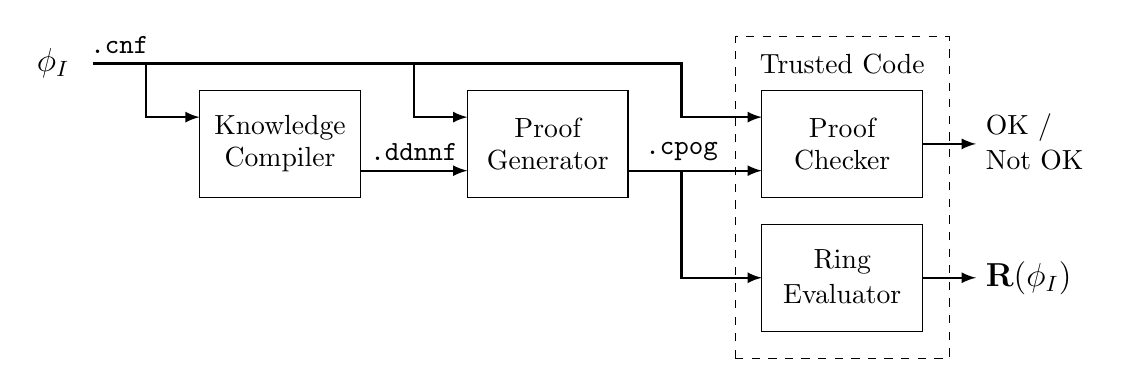
\begin{tikzpicture}[scale=0.17]
  \draw (8,10) rectangle (20,18);
  \node at (14,15.2) {Knowledge};
  \node at (14,12.8) {Compiler};

  \draw (28,10) rectangle (40,18);
  \node at (34,15.2) {Proof};
  \node at (34,12.8) {Generator};


  \draw (50,10) rectangle (62,18);
  \node at (56,15.2) {Proof};
  \node at (56,12.8) {Checker};

  \draw (50,0) rectangle (62,8);
  \node at (56,5.2) {Ring};
  \node at (56,2.8) {Evaluator};

  \draw[dashed] (48,-2) rectangle (64,22);
  \node at (56,20) {Trusted Code};

  %% CNF
  \draw[thick] (0,20) -- (44,20) -- (44,16) [-latex] -- (50,16);
  \draw[thick] (4,20) -- (4,16) [-latex] -- (8,16);
  \draw[thick] (24,20) -- (24,16) [-latex] -- (28,16);
  \node [left] at (-1,20) {\large {$\inputformula$}};
  \node [above] at (2,20) {\texttt{.cnf}};

  %% NNF
  \draw[thick] (20,12) [-latex] -- (28,12);
  \node [above] at (24,12) {\texttt{.ddnnf}};

  %% CPOG
  \draw[thick] (40,12) [-latex] -- (50,12);
  \draw[thick] (44,12) -- (44,4) [-latex] -- (50,4);
  \node [above] at (44,12) {\texttt{.cpog}};

  %% OK/Not
  \draw[thick] (62,14) [-latex] -- (66,14) ;
  \node [right] at (66,15.2) { OK /} ;
  \node [right] at (66,12.8) { Not OK} ;
  \draw[thick] (62,4) [-latex] -- (66,4) ;
  \node [right] at (66,4) {\large {$\textbf{R}(\inputformula)$}};

\end{tikzpicture}
}
\caption{Certifying toolchain.
  The output of a standard knowledge compiler is converted into a combined graph/proof (CPOG)
  which can be independently checked and evaluated}
\label{fig:chain}
\end{figure}

Figure~\ref{fig:chain} illustrates our certifying knowledge
compilation and model counting toolchain.  Starting with
input formula $\inputformula$, the \dfour{} knowledge compiler~\cite{lagniez:ijcai:2017}
generates a dec-DNNF representation,
and the \emph{proof
  generator} uses this to generate a CPOG file.
The \emph{proof checker} verifies the equivalence of the CNF and CPOG representations.
The \emph{ring evaluator} computes
a standard or weighted model count from the POG\@ representation.
As the dashed box in Figure~\ref{fig:chain} indicates, this toolchain
moves the root of trust away from the complex and highly
optimized knowledge compiler to a relatively simple checker and
evaluator.  Importantly, the proof generator need not be
trusted---its errors will be caught by the proof checker.

To ensure soundness of the abstract CPOG proof system, as well as
correctness of its concrete implementation, we formally verified the
proof system as well as versions of the proof checker and ring
evaluator in the \lean{} proof assistant~\cite{demoura:cade:2021}.
Running these two programs on a  CPOG file gives strong
assurance that the proof and the model count are correct. Our
experience with developing a formally verified proof checker has shown
that, even within the well-understood framework of extended
resolution, it can be challenging to formulate a full set of
requirements that guarantee soundness.  In fact, our efforts to
formally verify our proof framework exposed subtle conditions that we had
to impose on our partitioned sum rule.

We evaluate our toolchain using benchmark formulas from the 2022
standard and weighted model competitions.  Our tools handle all but
the largest dec-DNNF graphs generated by \dfour{}.  We also measure
the benefits of several optimizations as well as the relative
performance of the verified checker with one designed for high
performance and capacity.

We also show that our tools can provide end-to-end verification of
formulas that have been transformed by an equivalence-preserving
preprocessor.  That is, verification is based on the original formula,
and so proof checking certifies correct operation of the preprocessor,
the knowledge compiler, and the proof generator.

We have developed an online supplement to this
paper~\cite{bryant:sat:2023:supplement} that includes
a worked example, more details on the algorithms,
and extensive experimental results.  

\section{Related Work}


Generating proofs of unsatisfiability in SAT solvers has a long
tradition~\cite{ZhangMalik} and has become widely accepted due to the
formulation of clausal proof systems for which proofs can readily be
generated and efficiently checked
\cite{heule:cade:2013,wetzler14_drattrim}.
A number of formally verified checkers have been developed within different verification frameworks~\cite{cruz-cade-2017,lrat,Lammich:20,Tan:2021}.
The associated proofs add clauses while preserving satisfiability until the empty clause is derived.
Our work builds on the well-established technology and tools associated with clausal proof systems,
but we require features not found in proofs of unsatisfiability.
Our proofs construct a new propositional formula, and we must verify
both
that it
satisfies a set of rules and that it
is equivalent to the input formula.  This requires verifying
additional proof steps, including clause deletion steps, and subtle
invariants, as described in Sections~\ref{sect:cpog} and
\ref{section:formally-verified-toolchain}.

Capelli, Lagniez, and Marquis developed a knowledge compiler that
generates a certificate in a proof system that is itself based on
dec-DNNF~\cite{capelli:sat:2019,capelli:aaai:2021}.  Their \cdfour{}
program, a modified version of \dfour{}, generates annotations to the
compiled representation, providing information about how the compiled
version relates to the input clauses.  It also generates a file of
clausal proof steps in the DRAT format~\cite{wetzler14_drattrim}.
Completing the certification involves running two different checkers
on the annotated dec-DNNF graph and the DRAT file.  Although the
authors make informal arguments regarding the soundness of their
frameworks, these do not provide strong levels of assurance.  Indeed,
we have identified a weakness in their methodology due to an
invalid assumption about the guarantees provided by \dtrim{}, the
program it uses to check the DRAT file.  This weakness is
\emph{exploitable}: their framework can be ``spoofed'' into accepting
an incorrect compilation.

In more detail, \cdfour{} emits a sequence of clauses $R$ that
includes the conflict clauses that arose during a top-down processing of
the input clauses.  Given input formula $\phi_I$, their first task is to
check whether $\phi_I \imply R$, i.e., that any assignment that satisfies $\phi_I$ also satisfies each of the clauses in $R$.
They then base other parts of their proof on that
property and use a separate program to perform a series of additional
checks.  They use \dtrim{} to prove the implication, checking that each clause in $R$
satisifies the \emph{reverse asymmetric tautology} (RAT) property with
respect to the preceding
clauses~\cite{heule:cade:2013,jarvisalo:ijcar:2012}.  Adding a RAT
clause $C$ to a set of clauses maintains satisfiability, but it does not necessarily
preserve models.  As an example, consider the following formulas:
\begin{center}
  \begin{tabular}{lccc}
    $\phi_1$: & $(x_1 \lor x_3)$ & & \\
    $\phi_2$: & $(x_1 \lor x_3)$ & $\land$ & $(x_2 \lor \obar{x}_3)$\\
  \end{tabular}
\end{center}
Clearly, these two formulas are not equivalent---$\phi_1$ has six
models, while $\phi_2$ has four.  In particular, $\phi_1$ allows
arbitrary assignments to variable $x_2$.  Critically, however, the
second clause of $\phi_2$ is RAT with respect to $\phi_1$---any
satisfying assignment to $\phi_1$ can be transformed into one that
also satisfies $\phi_2$ by setting $x_2$ to 1, while keeping the values for other variables fixed.

This weakness would allow a buggy (or malicious) version of \cdfour{}
to spoof the checking framework.  Given formula $\phi_1$ as input, it
could produce a compiled result, including annotations, based on $\phi_2$ and also include the second clause of $\phi_2$ in $R$.
The check with \dtrim{} would pass, as would the other tests performed
by their checker.  We have confirmed this possibility with
their compiler and checker.\footnote{Downloaded May 18, 2023 as\\
\url{https://github.com/crillab/d4/tree/333370cc1e843dd0749c1efe88516e72b5239174}.}


This weakness can be corrected by restricting \dtrim{} to only add
clauses that obey the stronger \emph{reverse unit propagation} (RUP) property~\cite{goldberg,vangelder08_verifying_rup_proofs}.  We have added a
command-line argument to \dtrim{} that enforces this
restriction.\footnote{Available at
\url{https://github.com/marijnheule/drat-trim/releases/tag/v05.22.2023}.}  This weakness, however, illustrates the general challenge of
developing a new proof framework.
As we can attest,
without engaging in an effort to formally verify the framework, there are likely to be
conditions that make the framework unsound.

Fichte, Hecher, and Roland~\cite{fichte:sat:2022} devised the MICE
proof framework for model counting programs.  Their proof rules are
based on the algorithms commonly used by model counters.  They
developed a program that can generate proof traces from dec-DNNF
graphs and a program to check adherence to their proof rules.  This
framework is not directly comparable to ours, since it only certifies
the unweighted model count, but it has similar goals.
Again, they provide only  informal arguments
regarding the soundness of their framework.

Both of these prior certification frameworks are strongly tied to the
algorithms used by the knowledge compilers and model counters.  Some
of the conditions to be checked are relevant only to specific
implementations.    Our framework is very general and is based on a small set
of proof rules.  It builds on the highly developed
concepts of clausal proof systems.  These factors were important in enabling formal verification.
In Section~\ref{sect:experimental} and the supplement~\cite{bryant:sat:2023:supplement},
we also compare the performance of our toolchain to these other two.


\section{Logical Foundations}
\label{section:logical:foundations}

  Let $\varset$ denote a set of Boolean variables, and let $\assign$
  be an \emph{assignment} of truth values to some subset of the
  variables, where $0$ denotes false and $1$ denotes true, i.e.,
  $\assign \colon \varset' \rightarrow \{0,1\}$ for some $\varset'
  \subseteq \varset$.  We say the assignment is \emph{total} when it
  assigns a value to every variable ($\varset' = \varset$), and that
  it is \emph{partial} otherwise.
  The set of all possible total assignments over
  $\varset$ is denoted $\uassign$.

For each variable $x \in \varset$,
  we define the \emph{literals} $x$ and $\obar{x}$, where $\obar{x}$ is the
  negation of $x$. An
  assignment $\assign$ can be viewed as a set of literals, where
  we write $\lit \in \assign$ when $\lit = x$ and $\assign(x) = 1$ or when
  $\lit = \obar{x}$ and $\assign(x) = 0$.  We write the negation of literal $\lit$ as $\obar{\lit}$.  That is, $\obar{\lit} = \obar{x}$ when $\lit = x$ and
$\obar{\lit} = x$ when $\lit = \obar{x}$.


\begin{dfn}
  The set of Boolean formulas is defined recursively.  Each
  formula $\phi$ has an associated \emph{dependency set}
  $\dependencyset(\phi)  \subseteq \varset$, and a set of \emph{models} $\modelset(\phi)$,
  consisting of total assignments that satisfy the formula:
  \begin{enumerate}
  \item Boolean constants $0$ and $1$ are Boolean formulas,
    with $\dependencyset(0) = \dependencyset(1) = \emptyset$, with $\modelset(0) = \emptyset$, and with $\modelset(1) = \uassign$.
  \item Variable $x$ is a Boolean formula, with $\dependencyset(x) = \{x\}$
    and $\modelset(x) = \{\assign \in \uassign | \assign(x)=1\}$.
  \item For formula $\phi$, its \emph{negation}, written $\boolnot \phi$ is a Boolean formula,
    with $\dependencyset(\boolnot \phi) = \dependencyset(\phi)$ and $\modelset(\boolnot \phi) = \uassign - \modelset(\phi)$.
  \item For formulas $\phi_1, \phi_2, \ldots, \phi_k$, their \emph{product} $\phi = \bigwedge_{1 \leq i \leq k} \phi_i$ is a Boolean formula, with
      $\dependencyset(\phi) = \bigcup_{1 \leq i \leq k} \dependencyset(\phi_i)$ and
      $\modelset(\phi) = \bigcap_{1 \leq i \leq k} \modelset(\phi_i)$.
  \item For formulas $\phi_1, \phi_2, \ldots, \phi_k$, their \emph{sum} $\phi = \bigvee_{1 \leq i \leq k} \phi_i$ is a Boolean formula, with
      $\dependencyset(\phi) = \bigcup_{1 \leq i \leq k} \dependencyset(\phi_i)$ and
      $\modelset(\phi) = \bigcup_{1 \leq i \leq k} \modelset(\phi_i)$.
  \end{enumerate}
\label{def:boolean}
\end{dfn}


  We highlight some special classes of Boolean formulas.  A formula is
  in \emph{negation normal form} when negation is applied only to variables.  A
  formula is in \emph{conjunctive normal form} (CNF) when i) it is in
  negation normal form, and ii) sum is applied only to literals.  A CNF
  formula can be represented as a set of \emph{clauses}, each of which is a
  set of literals.  Each clause represents the sum of the
  literals, and the formula is the product of its clauses.  We use
  set notation to reference the clauses within a formula and the
  literals within a clause.  A clause consisting of a single literal is referred to as a \emph{unit} clause and the literal as a \emph{unit} literal.
This literal must be assigned value $1$ by any satisfying assignment of the formula.

\begin{dfn}
  \label{def:partitioned-operation-formula}
  A \emph{partitioned-operation formula}
 satisfies the following for all product and sum operations:
      \begin{enumerate}
      \item The arguments to each product must have disjoint dependency sets.  That is, operation
        $\bigwedge_{1 \leq i \leq k} \phi_i$ requires $\dependencyset(\phi_i) \cap \dependencyset(\phi_j) = \emptyset$ for $1 \leq i < j \leq k$.
      \item The arguments to each sum must have disjoint models.  That is, operation
        $\bigvee_{1 \leq i \leq k} \phi_i$ requires $\modelset(\phi_i) \cap \modelset(\phi_j) = \emptyset$ for $1 \leq i < j \leq k$.
      \end{enumerate}
\end{dfn}
     We let $\pand$ and $\por$ denote the product and sum operations in a partitioned-operation formula.

  \section{Ring Evaluation of a Boolean Formula}

We propose a general framework for summarizing properties of Boolean
formulas along the lines of algebraic model counting~\cite{kimmig:jal:2017}.

\begin{dfn}
  A \emph{commutative ring} $\ring$ is an algebraic structure
  $\langle \dset, \radd, \rmul, \addident, \mulident \rangle$,
  with elements in the set $\dset$ and with commutative and
  associative operations $\radd$ (addition) and $\rmul$ (multiplication),
  such that multiplication distributes
  over addition.  $\addident$ is the additive identity and $\mulident$ is
  the multiplicative identity.  Every element $a \in \dset$ has an
  \emph{additive inverse} $-a$ such that $a + -a = \addident$.
\label{def:ring}
\end{dfn}
We write $a - b$ as a shorthand for $a + -b$.

\begin{dfn}[Ring Evaluation Problem]
\label{def:ring_evaluation}
  For commutative ring $\ring$, a \emph{ring weight function} associates a value $w(x) \in \dset$ with
  every variable $x \in \varset$.  We then define $w(\obar{x}) \doteq \mulident-w(x)$.

  For Boolean formula $\phi$ and ring weight function $w$, the \emph{ring evaluation problem} computes
  \begin{equation}
    \begin{array}{rcl}
    \rep(\phi, w) & = & \sum_{\alpha \in \modelset(\phi)} \;\; \prod_{\lit \in \alpha} w(\ell) \label{eqn:rep}
    \end{array}
  \end{equation}
  In this equation, sum \scalebox{0.8}{$\sum$} is computed using addition operation $\radd$, and product \scalebox{0.8}{$\prod$} is computed using multiplication operation $\rmul$.
\label{def:weight}
\end{dfn}

Many important properties of Boolean formulas can be
expressed as ring evaluation problems.  The
(standard) \emph{model counting} problem for formula $\phi$ requires determining $|\modelset(\phi)|$.
It can be cast as a ring evaluation problem by having $\radd$ and
$\rmul$ be addition and multiplication over rational numbers and using
weight function $w(x) = 1/2$ for every variable $x$.
Ring evaluation of formula $\phi$ gives the \emph{density} of
the formula, i.e., the fraction of all possible total assignments that are
models.  For $n = |\varset|$, scaling the density by $2^n$
yields the number of models.

The \emph{weighted model counting}  problem is also defined over
rational numbers.  Some formulations  allow
independently assigning weights $W(x)$ and $W(\obar{x})$ for each variable $x$ and its complement, with the possibility that
$W(x) + W(\obar{x}) \not = 1$.
We can cast this as a
ring evaluation problem by letting $r(x) = W(x) + W(\obar{x})$,
performing ring evaluation with weight function $w(x) = W(x)/r(x)$ for each
variable $x$, and computing the weighted count
as $\rep(\phi, w)\; \rmul\; \prod_{x \in \varset} r(x)$.
Of course, this requires that $r(x) \not = 0$ for all $x \in \varset$.

The \emph{function hashing problem} provides a test
of inequivalence for Boolean formulas.  That is, for $n = |\varset|$, let $\ring$ be a
finite  field with $|\dset| = m$ such that $m \geq 2 n$.  For each $x \in \varset$, choose a value from $\dset$ at random for $w(x)$.  Two formulas
$\phi_1$ and $\phi_2$ will clearly have $\rep(\phi_1, w) = \rep(\phi_2, w)$
if they are logically equivalent,
and if $\rep(\phi_1, w) \not = \rep(\phi_2, w)$, then they are clearly inequivalent.
If they are not equivalent, then
the probability that $\rep(\phi_1, w) \not = \rep(\phi_2, w)$ will be at
least $\left(1-\frac{1}{m}\right)^n \geq \left(1-\frac{1}{2n}\right)^n > 1/2$.
Function hashing can therefore be used as part of a
randomized algorithm for equivalence testing~\cite{blum:ipl:1980}.
For example, it can compare different runs on a single formula,
either from different compilers or from a single compiler with different configuration parameters.


\section{Partitioned-Operation Graphs (POGs)}
\label{sect:pog}

Performing ring evaluation on an arbitrary Boolean formula could be intractable, but it is straightforward for a formula with partitioned operations:
\begin{prop}
\label{prop:ring:eval}
Ring evaluation with operations $\boolnot$, $\pand$, and $\por$ satisfies the following for any weight function $w$:
\begin{displaymath}
\begin{array}{rcl}
\rep(\boolnot \phi,\; w) &=& \mulident - \rep(\phi, w) \\
\textstyle
\scalebox{1.2}{\rep}\left(\Pand_{1 \leq i \leq k} \phi_i,\; w \right) &=& \prod_{1 \leq i \leq k} \rep(\phi_i, w) \\
\textstyle
\scalebox{1.2}{\rep}\left(\Por_{1 \leq i \leq k} \phi_i,\; w\right) &=& \sum_{1 \leq i \leq k} \rep(\phi_i, w) \\
\end{array}
\end{displaymath}
\end{prop}
As is described in \ref{section:formally-verified-toolchain}, we have proved these three equations using \lean{}.

A \emph{partitioned-operation graph} (POG) is a directed, acyclic
graph with nodes $N$ and edges $E \subseteq N \times N$.  We denote
nodes with boldface symbols, such as $\nodeu$ and $\nodev$.  When
$(\nodeu,\nodev) \in E$, node $\nodev$ is said to be a \emph{child} of
node $\nodeu$.  The in- and out-degrees of node $\nodeu$ are defined
as $\indegree(\nodeu) = | E \cap (N \times \{\nodeu\}) |$, and
$\outdegree(\nodeu) = | E \cap (\{\nodeu\} \times N) |$.  Node
$\nodeu$ is said to be \emph{terminal} if $\outdegree(\nodeu) = 0$.  A
terminal node is labeled by a Boolean constant or variable.  Node
$\nodeu$ is said to be \emph{nonterminal} if $\outdegree(\nodeu) > 0$.
A nonterminal node is labeled by Boolean operation $\pand$ or $\por$.
A node can be labeled with operation $\pand$ or $\por$ only if it
satisfies the partitioning restriction for that operation.  Every POG
has a designated \emph{root node} $\noder$.  Each edge has
a \emph{polarity}, indicating whether (negative polarity) or not
(positive polarity) the corresponding argument should be negated.

A POG represents a partitioned-operation
formula with a sharing of common subformulas.  Every node in the graph can be viewed as a partitioned-operation formula, and so we write
$\phi_{\nodeu}$ as the formula denoted by node $\nodeu$.
Each such formula has a set of models, and we write $\modelset(\nodeu)$ as a shorthand for $\modelset(\phi_{\nodeu})$.

We can now define and compare two related representations:
\begin{itemize}
\item A det-DNNF graph can be viewed a POG with negation applied only to variables.
\item A dec-DNNF graph is a det-DNNF graph with the further restriction that any
  sum node $\nodeu$ has exactly two children $\nodeu_1$ and $\nodeu_0$, and for these there is a \emph{decision variable} $x$ such that
  any total assignment $\assign \in  \modelset(\nodeu_b)$ has $\assign(x)=b$, for $b \in \{0,1\}$.
\end{itemize}
The generalizations encompassed by POGs have also been referred to as \emph{deterministic decomposable circuits} (d-Ds)~\cite{monet:amw:2018}.
Our current proof generator only works for knowledge compilers
generating dec-DNNF representations, but these generalizations
allow for future extensions, while maintaining the ability to
efficiently perform ring evaluation.


We define the \emph{size} of POG $P$, written $|P|$, to be the
the number of nonterminal nodes plus the number of edges from these nodes to their children.  Ring
evaluation of $P$ can be performed with at most $|P|$ ring
operations by traversing the graph from the terminal nodes up to
the root, computing a value $\rep(\nodeu, w)$ for each node $\nodeu$.
The final result is then $\rep(\noder, w)$.


Kimmig's formulation of algebraic model
counting~\cite{kimmig:jal:2017} is more general of ours.  It allows
the algebraic structure to be a \emph{semiring}, i.e., there need not
be additive inverses.  For example, it can have the sum operation be
$\max$ and the product operation be addition over the real numbers plus $\infty$.  This more general form
requires that the representation generated by the knowledge compiler
obey a property known as \emph{smoothness}~\cite{darwiche:jair:2002}.
Within our formulation, a partitioned-operation formula is smooth when
all arguments to each sum operation have identical dependency sets.
That is, every sum operation $\bigvee_{1 \leq i \leq k} \phi_i$ has
$\dependencyset(\phi_i) = \dependencyset(\phi_j)$ for $1 \leq i < j \leq k$.
Smoothness can be ensured by adding redundant formulas to
artificially introduce variables.  For example, if subformula $\phi_i$
lacks having variable $x$ in its dependency set, it can be replaced by
$(x \por \obar{x}) \pand \phi_i$.  The consideration of smoothness is
orthogonal to the issues addressed by this paper.  Given a smoothed
dec-DNNF graph generated by a knowledge compiler, our toolchain will
convert this into a smooth POG and verify its equivalence to the input
formula.

\section{Clausal Proof Framework}

We write (possibly subscripted) $\theta$ for
formulas encoded as clauses, possibly with extension variables.
We write (possibly subscripted)
$\phi$ for formulas
that use no extension variables.

A proof in our framework consists of a sequence of clause addition
and deletion steps, with each step preserving the set of solutions to
the original formula.
The status of the proof at any step is represented as
a set of \emph{active} clauses $\theta$, i.e., those that
have been added but not yet deleted.
Our framework is based
on \emph{extended} resolution~\cite{Tseitin:1983}, where proof
steps can introduce new \emph{extension variables} encoding Boolean formulas over input and prior extension variables.
Let $Z$
denote the set of extension variables occuring in formula $\theta$.
Starting with  $\theta$ equal to input formula $\inputformula$,
the proof must maintain the invariant that
$\inputformula \ifandonlyif \exists Z\,\theta$.

Clauses can be added in two different ways.  One is when they serve as
the \emph{defining clauses} for an extension variable.  This form
occurs only when defining $\pand$ and $\por$ operations, as is
described in Section~\ref{sect:cpog}.  Clauses can also be added or
deleted based on \emph{implication redundancy}.  That is, when clause
$C$ satisfies $\theta \imply C$ for formula $\theta$, then it can either
be added to $\theta$ to create the formula $\theta \cup \{C\}$ or it can be deleted
from $\theta \cup \{C\}$ to create $\theta$.

We use \emph{reverse unit propagation} (RUP) to certify
implication redundancy when adding or deleting
clauses~\cite{goldberg,vangelder08_verifying_rup_proofs}.
RUP
is the core rule supported by standard
proof checkers~\cite{heule:cade:2013,wetzler14_drattrim} for propositional logic. It provides a simple and efficient
way to check a sequence of applications of the resolution proof rule~\cite{robinson-1965}.
Let $C = \{\lit_1, \lit_2, \ldots,\lit_p\}$ be a clause to be
proved redundant with respect to formula $\theta$.  Let $D_1, D_2, \ldots, D_k$ be a sequence of supporting
\emph{antecedent} clauses, such that each $D_i$ is in $\theta$.
A RUP step
proves that $\bigwedge_{1\leq i \leq k} D_i \imply C$ by showing
that the combination of the antecedents plus the negation of $C$ leads
to a contradiction.  The negation of $C$ is the formula
$\overline{\lit}_1 \land \overline{\lit}_2 \land \cdots \land
\overline{\lit}_p$, having a CNF representation consisting of $p$ unit
clauses of the form $\obar{\lit}_i$ for $1 \leq i \leq p$.  A RUP
check processes the clauses of the antecedent in sequence, inferring
additional unit clauses.  In processing clause $D_i$, if all but one
of the literals in the clause is the negation of one of the
accumulated unit clauses, then we can add this literal to the
accumulated set.  That is, all but this literal have been falsified,
and so it must be set to true for the clause to be satisfied.  The
final step with clause $D_k$ must cause a contradiction, i.e., all of
its literals are falsified by the accumulated unit clauses.

Compared to the proofs of unsatisfiability generated by SAT solvers,
ours have important differences.  Most
significantly, each proof step must preserve the set of solutions with respect to the input variables;
our proofs must therefore justify both clause deletions and additions.
By contrast, an unsatisfiability proof need only guarantee that
no proof step causes a satisfiable set of clauses to become
unsatisfiable, and therefore it need only justify clause additions.


\section{The CPOG Representation and Proof System}
\label{sect:cpog}


%% The proof system is based on extended
%% resolution~\cite{Tseitin:1983} with reverse unit propagation
%% (RUP)~\cite{goldberg,vangelder08_verifying_rup_proofs} as the core method for
%% proving that a set of clauses logically implies another clause.
%% Alternate version
%% knowledge compilation.  The proof system is based on extended
%% resolution~\cite{Tseitin:1983} with reverse unit propagation
%% (RUP)~\cite{goldberg,vangelder08_verifying_rup_proofs} as the core method for
%% proving that a set of clauses logically implies another clause.
%%
%% As an example, consider the formula $\varphi = (\obar{a} \lor b) \land (\obar{b} \lor c \lor \obar{e}) \land (\obar c \lor d)$
%% and a RUP step to derive the target clause $(\obar{a} \lor d \lor \obar{e})$ from the three clauses from $\varphi$.
%% A RUP proof would take the following form.  We start with the assignment that falsifies the target clause. This assignment
%% is extended by clauses in $\varphi$ that become unit and eventually the empty clause. In the illustration below, the
%% involved clauses (antecedents) are shown in the order that they became unit / falsified.
%%
%% \begin{center}
%%   \begin{tabular}{lcccc}
%%          & \makebox[15mm]{Target}    & \makebox[10mm]{} & \makebox[10mm]{Antecedents} & \makebox[10mm]{} \\
%%   Clause & $\obar{a} \lor d \lor \obar{e}$ & $\obar{c} \lor d$  & $\obar{e} \lor \obar{b} \lor c$   & $\obar{a} \lor b$ \\
%%   \midrule
%%   Units  & $a$, $\obar{d}$, $e$      &  $\obar{c}$             & $\obar{b}$                         & $\nil$ \\
%%   \end{tabular}
%% \end{center}
%%
%% RUP is an alternative formulation of resolution.  For target clause
%% $C$, it can be seen that applying resolution operations to the
%% antecedent clauses from right to left will derive a clause $C'$ such
%% that $C' \subseteq C$.  By \emph{subsumption} %~\cite{philipp:lpar:2017},
%% we then have $C' \rightarrow C$.  Compared to listing each resolution
%% operation as a separate step, using RUP as the basic proof step makes
%% the proofs more compact.
%%
%% As is shown in Figure~\ref{fig:chain}
%% two programs are involved in producing a certified compilation of a formula:
%% \begin{itemize}
%% \item The \emph{proof generator} produces a CPOG file that both defines the POG and gives a proof that the POG is logically equivalent to the input formula.
%% As the figure indicates, the generator starts with the output of another knowledge compiler, such as one generating a dec-DNNF representation of the formula.
%% \item The \emph{proof checker} ensures that all of the proof conditions are satisfied.
%% \end{itemize}
%% >>>>>>> 9c1793da858d00e5d4022d6d33c009848ba2083b

A CPOG file provides both a declaration of a POG, as well as a checkable
proof that a Boolean formula, given in conjunctive normal
form, is logically equivalent to the POG\@.
The proof format draws its inspiration from the LRAT~\cite{lrat} and
QRAT~\cite{heule:JAR2014} formats for unquantified and quantified Boolean formulas, respectively.
Key properties include:
\begin{itemize}
  \item
  The file contains declarations of $\pand$ and $\por$ operations to describe the POG.
  Declaring a node $\nodeu$ implicitly adds an \emph{extension} variable $u$ and a set of \emph{defining} clauses $\theta_{u}$
  encoding the product or sum operation.
  This is the only means for adding extension variables to the proof.
\item Boolean negation is supported implicitly by allowing the
  arguments of the $\por$ and $\pand$ operations to be literals and not just
  variables.
\item
  The file contains explicit clause addition steps.
  A clause can only be added if it is logically implied by the existing clauses.
  A sequence of clause identifiers must be listed as a \emph{hint} providing a RUP verification of the implication.
\item
  The file contains explicit clause deletion steps.
  A clause can only be deleted if it is logically implied by the remaining clauses.
  A sequence of clause identifiers must be listed as a \emph{hint} providing a RUP verification of the implication.
\item The checker must track the dependency set for every input and
  extension variable.  For each $\pand$ operation, the checker must ensure that the dependency sets for its arguments are disjoint.
  The associated extension variable has a dependency set equal to the union of those of its arguments.
\item Declaring a $\por$ operation requires a sequence of clauses
  providing a RUP proof that the arguments are mutually exclusive.
  Only binary $\por$ operations are allowed to avoid requiring multiple proofs of disjointness
%  Generalizing to $k$ arguments would require
%  $k\,(k-1)/2$ proofs of disjointness.
\end{itemize}

\subsection{Syntax}
\label{subsection:syntax}

\begin{table}
  \caption{CPOG Step Types.  $C$: clause identifier, $L$: literal, $V$: variable}
  \label{tab:cpog:syntax}
\centering{
  \begin{tabular}{lllll}
    \toprule
    \multicolumn{4}{c}{Rule} & \multicolumn{1}{c}{Description} \\
    \midrule
    \makebox[5mm][l]{$C$} & \makebox[10mm][l]{\texttt{a}}  & \makebox[15mm][l]{$L^{*}$ \texttt{0}} & \makebox[15mm][l]{$C^{+}$ \texttt{0}}  & \makebox[20mm][l]{Add RUP clause} \\
     & \texttt{d} & $C$             & $C^{+}$  \texttt{0} & Delete RUP clause \\
    \midrule
    $C$    & \texttt{p} & $V \; L^{*}$ \texttt{0}    &                  & Declare $\pand$ operation \\
    $C$    & \texttt{s} & $V \; L \; L$    & $C^{+}$ \texttt{0}  & Declare $\por$ operation \\
    \midrule
     & \texttt{r} & $L$             &            & Declare root literal\\
    \bottomrule
  \end{tabular}
  }
\end{table}

Table~\ref{tab:cpog:syntax} shows the declarations that can occur in a CPOG file.
%% The checker is provided with the input formula as a separate file.
As with other clausal proof formats, a variable is
represented by a positive integer $v$, with the first ones being input
variables and successive ones being extension variables.  Literal $\lit$
is represented by a signed integer, with $-v$ being the logical negation of
variable $v$.  Each clause is indicated by a positive integer
identifier $C$, with the first ones being the IDs of the input clauses and successive
ones being the IDs of added clauses.  Clause identifiers must be totally ordered,
such that any clause identifier $C'$ given in the hint when adding clause $C$ must have $C' < C$.

The first set of proof rules are similar to those in other clausal
proofs.
Clauses can be added via RUP addition
(command \texttt{a}), with a sequence of antecedent clauses (the
``hint'').
Similarly for clause deletion (command \texttt{d}).

\begin{table}
\caption{Defining Clauses for Product (A) and Sum (B) Operations}
\begin{minipage}{0.54\textwidth}
\begin{center}
\begin{tabular}{cccccc}
\multicolumn{6}{c}{(A).  Product Operation $\pand$}\\
\toprule
\makebox[10mm]{ID} & \multicolumn{5}{c}{Clause} \\
\midrule
  $i$ & $v$ & $-\lit_1$ & $-\lit_2$ & $\cdots$ & $-\lit_k$\\
  $i\!+\!1$ & $-v$ & $\lit_1$  \\
  $i\!+\!2$ & $-v$ & $\lit_2$  \\
  & $\ldots$ \\
  $i\!+\!k$ & $-v$ & $\lit_k$  \\
\bottomrule
\end{tabular}
\end{center}
\end{minipage}
\begin{minipage}{0.44\textwidth}
\begin{center}
\begin{tabular}{cccc}
\multicolumn{4}{c}{(B).  Sum Operation $\por$}\\
\toprule
\makebox[10mm]{ID} & \multicolumn{3}{c}{Clause} \\
\midrule
  $i$ & $-v$ & $\lit_1$ & $\lit_2$ \\
  $i\!+\!1$ & $v$ & $-\lit_1$ \\
  $i\!+\!2$ & $v$ & $-\lit_2$ \\
\bottomrule
$\;$ \\
$\;$ \\
\end{tabular}
\end{center}
\end{minipage}
\label{tab:defining}
\end{table}

The declaration of a \emph{product} operation, creating a node with operation $\pand$,
 has the form:
\begin{center}
\begin{tabular}{ccccccccc}
  \makebox[5mm]{$i$} & \makebox[5mm]{\texttt{p}} & \makebox[5mm]{$v$} & \makebox[5mm]{$\lit_1$} & \makebox[5mm]{$\lit_2$} &
  \makebox[5mm]{$\cdots$} & \makebox[5mm]{$\lit_k$} & \makebox[5mm]{\texttt{0}} \\
\end{tabular}
\end{center}
Integer $i$ is a new clause ID, $v$ is a positive integer that does not
correspond to any previous variable, and $\lit_1, \lit_2, \ldots, \lit_k$ is a sequence of $k$
integers, indicating the arguments as literals of existing variables.
As Table~\ref{tab:defining}(A) shows,
this declaration implicitly causes $k+1$ clauses to be added to the proof, providing a Tseitin encoding that defines extension variable $v$ as the product of its arguments.

The dependency sets for the arguments represented by each pair of
literals $\lit_i$
and $\lit_{j}$ must
be disjoint, for $1 \leq i < j \leq k$.  A product operation may have no arguments,
representing Boolean constant $1$.  The only clause added to the proof will be
the unit literal $v$.  A reference to literal $-v$ then provides a way
to represent constant $0$.

The declaration of a \emph{sum} operation, creating a node with operation $\por$, has the form:
\begin{center}
\begin{tabular}{ccccccc}
  \makebox[5mm]{$i$} & \makebox[5mm]{\texttt{s}} & \makebox[5mm]{$v$} & \makebox[5mm]{$\lit_1$} & \makebox[5mm]{$\lit_2$}
\makebox[5mm]{$H$} & \makebox[5mm]{$\texttt{0}$} \\
\end{tabular}
\end{center}
Integer $i$ is a new clause ID, $v$ is a positive integer that does
not correspond to any previous variable, and $\lit_1$ and $\lit_2$ are
signed integers, indicating the arguments as literals of existing variables.  Hint $H$
consists of a
sequence of clause IDs, all of which must be defining clauses for other POG operations.\footnote{The restriction to defining clauses in the hint is critical to soundness.
Allowing the hint to include the IDs of input clauses creates an exploitable weakness.  We discovered this weakness in the course of our efforts at formal verification.}
As Table~\ref{tab:defining}(B) shows,
this declaration implicitly causes three clauses to be added to the proof, providing a Tseitin encoding that defines extension variable $v$ as the sum of its arguments.
The hint must provide a RUP proof of the clause $\obar{\lit}_1 \lor \obar{\lit}_2$, showing that the two children of this node have disjoint models.

Finally, the literal denoting the root of the POG is declared with the
\texttt{r} command.  It can occur anywhere in the file.  Except in degenerate cases, it
will be the extension variable representing the root of a graph.
%, but in
%degenerate cases it can be the positive or negative literal of an
%input variable.

\subsection{Semantics}
\label{subsection:semantics}

The defining clauses for a product or sum
operation uniquely define the value of its extension variable for any assignment of values to the argument variables.
For the
extension variable $u$ associated with any POG node $\nodeu$, we can therefore
prove that any total assignment $\assign$ to the input variables that
also satisfies the POG defining clauses will
assign a value to $u$ such that $\assign(u) =
1$ if and only if $\assign \in \modelset(\nodeu)$.

%% A CPOG proof follows the same general form as a QRAT dual
%% proof~\cite{bryant:cade:2021}---one that ensures that each clause
%% addition and each clause deletion preserves equivalence.  With CPOG,
%% however, clauses are defined both explicitly and implicitly.  Starting
%% with the set of input clauses, the proof consists of a sequence of
%% steps that both add and delete clauses.  Each addition must be truth
%% preserving, that is, any satisfying total assignment for the set of clauses
%% before clause addition should still be a satisfying assignment afterwards.
%% Each deletion must be falsehood preserving.  That is, there can be no
%% new satisfying assignments when the clause is deleted.

The sequence of operator declarations, asserted clauses, and
clause deletions represents a systematic transformation of the input formula
into a POG\@.  Validating all of these steps serves to prove that
POG $P$ is logically equivalent to the input formula.
At the completion of the proof, the following \textsc{final conditions} must hold:
\begin{enumerate}
\item There is exactly one remaining clause that was added via RUP
  addition, and this is a unit clause consisting of root literal $r$.
\item All of the input clauses have been deleted.
\end{enumerate}
In other words, at the end of the proof it must hold that the active clauses be exactly those
in $\pogformula \doteq \{\{r\}\} \cup \; \bigcup_{\nodeu \in P} \theta_{u}$, the formula consisting
of unit clause $\{r\}$ and the defining clauses for the nodes, providing a Tseitin encoding of $P$. Recognizing that
any total assignment to the input variables implicitly defines the assignments to the extension variables,
we can see that $\pogformula$ is the clausal encoding of $\phi_\noder$.
Let $\inputformula$ denote the input formula.
The sequence of clause addition steps provides a \emph{forward implication} proof that
$\modelset(\inputformula) \subseteq \modelset(\phi_\noder)$.  That is, any total
assignment $\assign$ satisfying the input formula must also satisfy
the formula represented by the POG\@.
Conversely,
each proof step that deletes an input clause proves that any
total assignment $\alpha$ that falsifies the clause must
falsify $\phi_\noder$.  Deleting all but the final asserted clause and all input clauses provides a \emph{reverse implication} proof
that
$\modelset(\phi_\noder) \subseteq \modelset(\inputformula)$.

\subsection{CPOG Example}
\label{sect:cpog:example}

\begin{figure}
\begin{minipage}{0.58\textwidth}
(A)  Input Formula\\[1.2ex]
\begin{tabular}{lll}
\toprule
\makebox[5mm]{ID} & \makebox[15mm]{Clauses} & \\
\midrule
1 & \texttt{-1 3 -4} & \texttt{0} \\
2 & \texttt{-1 -3 4} & \texttt{0} \\
3 & \texttt{3 -4} & \texttt{0}\\
4 & \texttt{1 -3 4} & \texttt{0} \\
5 & \texttt{-1 -2} & \texttt{0} \\
\bottomrule
\end{tabular}
\\[1.8ex]
(C) POG Declaration\\[1.2ex]
\begin{tabular}{llll}
\toprule
\makebox[5mm]{ID} & \multicolumn{2}{l}{CPOG line} & Explanation \\
\midrule
6 & \texttt{p 5 -3 -4} & \texttt{0} & $p_5 = \obar{x}_3 \pand \obar{x}_4$ \\
9 & \texttt{p 6 3 4} & \texttt{0} & $p_6 = x_3 \pand x_4$ \\
12 & \texttt{s 7 5 6 7 10} & \texttt{0} & $s_7 = p_5 \por p_6$ \\
15 & \texttt{p 8 -1 7} & \texttt{0} & $p_8 = \obar{x}_1 \pand s_7$ \\
18 & \texttt{p 9 1 -2 7} & \texttt{0} & $p_9 = x_1 \pand \obar{x}_2 \pand s_7$ \\
22 & \texttt{s 10 8 9 16 19} & \texttt{0} & $s_{10} = p_8 \por p_9$ \\
 & \texttt{r 10} && Root $r = s_{10}$\\
\bottomrule
\end{tabular}
\end{minipage}
\begin{minipage}{0.35\textwidth}
(B) POG Representation \\
\input{dd/eg4}
\end{minipage}
%% Break
\\[2.5ex]
\begin{minipage}{0.42\textwidth}
(D) Defining Clauses\\[1.2ex]
\begin{tabular}{llll}
\toprule
\makebox[5mm]{ID} & \multicolumn{2}{l}{Clauses} & Explanation \\
\midrule
\texttt{6} & \texttt{5 3 4} & \texttt{0} & Define $p_5$ \\
\texttt{7} & \texttt{-5 -3} & \texttt{0} & \\
\texttt{8} & \texttt{-5 -4} & \texttt{0} & \\
\midrule
\texttt{9} & \texttt{6 -3 -4} & \texttt{0} & Define $p_6$ \\
\texttt{10} & \texttt{-6 3} & \texttt{0} & \\
\texttt{11} & \texttt{-6 4} & \texttt{0} & \\
\midrule
\texttt{12} & \texttt{-7 5 6} & \texttt{0} & Define $s_7$ \\
\texttt{13} & \texttt{7 -5} & \texttt{0} & \\
\texttt{14} & \texttt{7 -6} & \texttt{0} & \\
\midrule
\texttt{15} & \texttt{8 1 -7} & \texttt{0} & Define $p_8$ \\
\texttt{16} & \texttt{-8 -1} & \texttt{0} & \\
\texttt{17} & \texttt{-8 7} & \texttt{0} & \\
\midrule
\texttt{18} & \texttt{9 -1 2 -7} & \texttt{0} & Define $p_9$ \\
\texttt{19} & \texttt{-9 1} & \texttt{0} & \\
\texttt{20} & \texttt{-9 -2} & \texttt{0} & \\
\texttt{21} & \texttt{-9 7} & \texttt{0} & \\
\midrule
\texttt{22} & \texttt{-10 8 9} & \texttt{0} & Define $s_{10}$ \\
\texttt{23} & \texttt{10 -8} & \texttt{0} & \\
\texttt{24} & \texttt{10 -9} & \texttt{0} & \\
\bottomrule
\end{tabular}
\end{minipage}
\begin{minipage}{0.49\textwidth}
(E) CPOG Assertions\\[1.2ex]
\begin{tabular}{llllll}
\toprule
\makebox[5mm]{ID} & \multicolumn{2}{l}{Clause} & \multicolumn{2}{l}{Hint} & Explanation \\
\midrule
\texttt{25} & \texttt{a 5 1 3} & \texttt{0} & \texttt{3 6} & \texttt{0} & $\obar{x}_1 \land \obar{x}_3 \imply p_5$ \\
\texttt{26} & \texttt{a 6 1 -3} & \texttt{0} & \texttt{4 9} & \texttt{0} & $\obar{x}_1 \land x_3 \imply p_6$ \\
\texttt{27} & \texttt{a 3 7 1} & \texttt{0} & \texttt{13 25} & \texttt{0} & $\obar{x}_3 \land \obar{x}_1 \imply s_7$  \\
\texttt{28} & \texttt{a 7 1} & \texttt{0} & \texttt{27 14 26} & \texttt{0} & $\obar{x}_1 \imply s_7$  \\
\texttt{29} & \texttt{a 8 1} & \texttt{0} & \texttt{28 15} & \texttt{0} & $\obar{x}_1 \imply p_8$  \\
\texttt{30} & \texttt{a 5 -1 3} & \texttt{0} & \texttt{1 6} & \texttt{0} & $x_1 \land \obar{x}_3 \imply p_5$ \\
\texttt{31} & \texttt{a 6 -1 -3} & \texttt{0} & \texttt{2 9} & \texttt{0} & $x_1 \land x_3 \imply p_6$ \\
\texttt{32} & \texttt{a 3 7 -1} & \texttt{0} & \texttt{13 30} & \texttt{0} & $\obar{x}_3 \land x_1 \imply s_7$  \\
\texttt{33} & \texttt{a 7 -1} & \texttt{0} & \texttt{32 14 31} & \texttt{0} & $x_1 \imply s_7$  \\
\texttt{34} & \texttt{a 9 -1} & \texttt{0} & \texttt{5 33 18} & \texttt{0} & $x_1 \imply p_9$  \\
\texttt{35} & \texttt{a 1 10} & \texttt{0} & \texttt{23 29} & \texttt{0} & $\obar{x}_1 \imply s_{10}$  \\
\texttt{36} & \texttt{a 10} & \texttt{0} & \texttt{35 24 34} & \texttt{0} & $s_{10}$ \\
\bottomrule
\end{tabular}
\\[1.5ex]
(F) Input Clause Deletions\\[1.2ex]
\begin{tabular}{lllll}
  \toprule
 \multicolumn{3}{l}{CPOG line} & Explanation\\
\midrule
 \texttt{d 1} & \texttt{36 8 10 12 16 21 22} & \texttt{0} & Delete clause 1 \\
 \texttt{d 2} & \texttt{36 7 11 12 16 21 22} & \texttt{0} & Delete clause 2 \\
 \texttt{d 3} & \texttt{36 8 10 12 17 19 22} & \texttt{0} & Delete clause 3 \\
 \texttt{d 4} & \texttt{36 7 11 12 17 19 22} & \texttt{0} & Delete clause 4 \\
 \texttt{d 5} & \texttt{36 16 20 22} & \texttt{0} &  Delete clause 5 \\
\bottomrule
\end{tabular}
\end{minipage}
\caption{Example formula (A), its POG representation (B), and its CPOG proof (C), (E), and (F)}
\label{fig:eg4:all}
\end{figure}

Figure \ref{fig:eg4:all} illustrates an example formula and shows how
the CPOG file declares its POG representation.  The input formula (A)
consists of five clauses over variables $x_1$, $x_2$, $x_3$, and
$x_4$.  The generated POG (B) has six nonterminal nodes representing
four products and two sums.  We name these by the node
type (product $\nodep$ or sum $\nodes$), subscripted by the ID of the
extension variable.
% We denote the extension variable for nodes $\nodep_i$ and $\nodes_j$ as $p_i$ and $s_j$, respectively.
  The first part of the CPOG file (C) declares
these nodes using clause IDs that increment by three or four,
depending on whether the node has two children or three.  The last two
nonzero values in the sum declarations are the hint providing the
required mutual exclusion proof.

\subsection{Node Declarations}

We step through portions of the file to provide a better understanding of the CPOG proof framework.
Figure
\ref{fig:eg4:all}(D) shows the defining clauses that are implicitly
defined by the POG operation declarations.  These do not appear in the
CPOG file.  Referring back to the declarations of the sum nodes in
Figure \ref{fig:eg4:all}(C), we can see that the declaration of node
$\nodes_7$ had clause IDs 7 and 10 as the hint.  We can see in Figure
\ref{fig:eg4:all}(A) that these two clauses form a RUP proof for the clause
$\obar{p}_5 \lor \obar{p}_6$, showing that the two children of $\nodes_7$
have disjoint models.  Similarly, node $\nodes_{10}$ is declared as having
clause IDs 16 and 19 as the hint.  These form a RUP proof for the clause
$\obar{p}_8 \lor \obar{p}_9$, showing that the two children of
$\nodes_{10}$ have disjoint models.

\subsection{Forward Implication Proof}

Figure \ref{fig:eg4:all}(E) provides the sequence of assertions
leading to unit clause 36, consisting of the literal $s_{10}$.  This clause indicates that $\nodes_{10}$ is implied by the input clauses, i.e.,
any total assignment $\assign$
satisfying the input clauses must have $\assign(s_{10}) = 1$.
Working backward, we can see that
clause 29 indicates that variable $p_8$ will be implied by the input
clauses when $\assign(x_1) = 0$, while clause 34 indicates that node $p_9$ will
be implied by the input clauses when $\assign(x_1) = 1$.  These serve as the
hint for clause 36.

\subsection{Reverse Implication Proof}

Figure \ref{fig:eg4:all}(F) shows the RUP proof steps required to
delete the input clauses.  Consider the first of these, deleting
input clause $\obar{x}_1 \lor x_3 \lor \obar{x}_4$.  The requirement is to show
that there is no total assignment $\assign$ that falsifies this clause but assigns $\assign(s_{10}) = 1$.
The proof proceeds by first assuming that the clause is false, requiring
$\assign(x_1) = 1$, $\assign(x_3) = 0$, and $\assign(x_4) = 1$.  The hint then consist of unit
clauses (e.g., clause 36 asserting that $\alpha(p_{10}) = 1$) or
clauses that cause unit propagation.  Hint clauses 8 and 10 force the
assignments $\assign(p_5) = \assign(p_6) = 0$.  These, plus hint clause 12 force
$\assign(s_7) = 0$.  This, plus hint clauses 16 and 21 force $\assign(p_8) = \assign(p_9) = 0$, leading,
via clause 22, to $\assign(s_{10}) = 0$.  But this contradicts clause 36,
completing the RUP proof.  The deletion hints for the other input
clauses follow similar patterns---they work from the bottom nodes of
the POG upward, showing that any total assignment that falsifies the clause
must assign $\assign(s_{10}) = 0$.

Deleting the asserted clauses is so simple that we do not show it.  It
involves simply deleting the clauses from clause number 35 down to
clause number 25, with each deletion using the same hint as were used
to add that clause.  In the end, therefore, only the defining clauses
for the POG nodes and the unit clause asserting $s_{10}$ remain,
completing a proof that the POG is logically equivalent to the input
formula.

\section{Generating CPOG from dec-DNNF}
\label{section:generating:cpog}

%%Figure~\ref{fig:chain} illustrates one method of generating a CPOG
%%file from an input formula in conjunctive normal form.  Our toolchain
%%is based on the \dfour{} knowledge compiler~\cite{lagniez:ijcai:2017},
%%but it would also work for other tools that use a top-down search
%%strategy to generate a dec-DNNF representation.
A dec-DNNF
graph can be directly translated  into a POG.
In doing this conversion,
our program performs simplifications to
eliminate Boolean constants.
Except in degenerate cases,
where the formula is unsatisfiable or a tautology,
we can therefore assume
that the POG does not contain any constant nodes.
In addition, negation is only
applied to variables, and so the only edges with negative polarity will have variables as children.
We can therefore
view the POG as consisting
of \emph{literal} nodes corresponding to input variables and their negations, along with
\emph{nonterminal} nodes, which can be further classified as \emph{product} and \emph{sum} nodes.

\subsection{Forward Implication Proof}

For input formula $\inputformula$ and its translation into a POG $P$
with root node $\noder$, the most challenging part of the proof is to
show that $\modelset(\inputformula) \subseteq \modelset(\phi_\noder)$, i.e.,
that any total assignment $\assign$ that is a model of $\inputformula$
and the POG definition clauses
will yield $\assign(r) = 1$, for root literal $r$.  This part of the
proof consists of a series of clause assertions leading to one adding
$\{r\}$ as a unit clause.  We have devised two methods for generating this
proof.  The \emph{monolithic} approach makes just one call to a
proof-generating SAT solver and has it determine the relationship
between the two representations.  The \emph{structural} approach
recursively traverses the POG, generating proof obligations at each
node encountered.  It may require multiple calls to a proof-generating SAT
solver.

As notation,
let $\psi$ be a subset of the clauses in $\inputformula$.
For partial assignment
$\passign$, the expression  $\simplify{\psi}{\passign}$ denotes the set of clauses $\gamma$
obtained from $\psi$ by: i) eliminating any
clause containing a literal $\lit$ such that $\passign(\lit) = 1$,
ii) for the remaining clauses eliminating those literals $\lit$ for
which $\passign(\lit) = 0$, and iii) eliminating any duplicate or tautological clauses.
In doing these simplifications, we also track the \emph{provenance}
of each simplified clause $C$, i.e., which of the (possibly multiple) input clauses simplified to become $C$.
More formally, for $C \in \simplify{\psi}{\passign}$, we let $\prov_{\passign}(C, \psi)$ denote
those clauses $C' \in \psi$, such that
$C' \subseteq C \cup \bigcup_{\lit \in \passign} \obar{\lit}$.
We then extend the definition of $\prov$ to any simplified formula
$\gamma$ as $\prov_{\passign}(\gamma, \psi) = \bigcup_{C \in \gamma} \prov_{\passign}(C, \psi)$.

The monolithic approach
takes advantage of the clausal representations of
the input formula $\inputformula$ and the POG formula $\phi_\noder$.
We can express the negation of $\phi_\noder$ in clausal form as
$\theta_{\obar{\noder}} \doteq \bigcup_{\nodeu\in P} \simplify{\theta_{u}}{\{\obar{r}\}}$.
Forward implication will hold when $\inputformula \imply \phi_\noder$, or  equivalently
when the formula $\inputformula \land \theta_{\obar{\noder}}$
is unsatisfiable, where the
conjunction can be expressed as the union
of the two sets of clauses.  The proof generator writes the clauses to a file and invokes a proof-generating SAT solver.
For each clause $C$ in the unsatisfiability proof, it adds clause $\{r\} \cup C$ to the CPOG proof, and so the empty clause in the proof becomes the unit clause $\{r\}$.
Our experimental results show
that this approach can be very effective and generates short proofs
for smaller problems, but it does not scale well enough for general
use.


The structural approach to proof generation takes the form of a recursive procedure
$\validate(\nodeu, \passign, \psi)$ taking as arguments POG
node $\nodeu$, partial assignment
$\passign$, and a set of clauses $\psi \subseteq \inputformula$.
The procedure adds a number of clauses to the proof, culminating with
the addition of the \emph{target} clause:
$u \lor \bigvee_{\lit \in \passign} \obar{\lit}$, indicating
that $(\bigwedge_{\lit \in \passign} \lit) \imply u$, i.e.,
that any total
assignment $\assign$ such that $\passign \subseteq \assign$
will assign $\assign(u) = 1$.
The top-level call has $\nodeu = \noder$, $\passign = \emptyset$, and $\psi = \inputformula$.
The result will therefore be to add unit clause $\{r\}$ to the proof.
Here we present a correct, but somewhat inefficient formulation of
$\validate$.  We then refine it with some optimizations.

The recursive call $\validate(\nodeu, \passign, \psi)$ assumes that we have
traversed a path from the root node down to node $\nodeu$, with the
literals encountered in the product nodes forming the partial
assignment $\passign$.  The set of clauses $\psi$ can be a proper
subset of the input clauses $\inputformula$ when a product node has caused
a splitting into clauses containing disjoint variables.
The subgraph with root node $\nodeu$ should be a POG representation of the formula
$\simplify{\psi}{\passign}$.
%% Having the
%% routine add its target clause indicates that any total assignment
%% $\assign$ such that $\passign \subseteq \assign$ will yield $\alpha(u) = 1$.

The process for generating such a proof depends on the form of node $\nodeu$:
\begin{enumerate}
\item If $\nodeu$ is a literal $\lit'$, then the formula
  $\simplify{\psi}{\passign}$ must consist of the single unit clause
  $C = \{\lit'\}$, such that any $C' \in \prov_{\passign}(C, \psi)$ must have $C' \subseteq \{ \lit' \} \cup\, \bigcup_{\lit \in \passign} \obar{\lit}$.
  Any of these can
  serve as the target clause.
\item If $\nodeu$ is a sum node with children $\nodeu_1$ and $\nodeu_0$,
  then, since the node originated from a dec-DNNF graph, there must be
  some variable $x$ such that either $\nodeu_1$ is a literal node for $x$ or $\nodeu_1$ is a
  product node containing a literal node for $x$ as a child.  In either case, we
  recursively call $\validate(\nodeu_1, \passign \cup \{ x \}, \psi)$.
  This will cause the addition of the target clause
  $u_1 \lor \obar{x} \lor \bigvee_{\lit \in \passign} \obar{\lit}$.
Similarly, either $\nodeu_0$ is a literal node for $\obar{x}$ or $\nodeu_0$ is a product node containing a literal node for $\obar{x}$ as
  a child.  In either case, we recursively call $\validate(\nodeu_0, \passign \cup \{ \obar{x} \}, \psi)$,
  causing the addition of the target clause
  $u_0 \lor x \lor \bigvee_{\lit \in \passign} \obar{\lit}$.
  These recursive results can be combined with the second and third defining clauses for $\nodeu$
(see Table~\ref{tab:defining}(B))
  to generate the target clause for $\nodeu$, requiring at most two RUP steps.
\item If $\nodeu$ is a product node, then we can divide its children
  into a set of literal nodes $\lambda$ and a set of nonterminal nodes $\nodeu_1, \nodeu_2, \ldots, \nodeu_k$.
  \begin{enumerate}
    \item For each literal
  $\lit \in \lambda$, we must prove that any total assignment $\alpha$, such that
  $\passign \subset \alpha$ has $\alpha(\lit) = 1$.  In some
  cases, this can be done by simple Boolean constraint propagation (BCP).
  In other cases, we must prove that the formula
  $\simplify{\psi}{\passign \cup \{\obar{\lit}\}}$ is unsatisfiable.  We
  do so by writing the formula to a file, invoking a proof-generating
  SAT solver, and then converting the generated unsatisfiability proof
  into a sequence of clause additions in the CPOG file.
  (The solver is constrained to only use RUP inference rules, preventing it from introducing extension variables.)
\item For a single nonterminal child ($k = 1$), we recursively call
  $\validate \left(\nodeu_1, \passign \cup \lambda, \psi\right)$.
\item For multiple nonterminal children ($k > 1$),
  it must be the case that the clauses in
  $\gamma = \simplify{\psi}{\passign}$ can be partitioned into $k$ subsets
  $\gamma_1, \gamma_2, \ldots, \gamma_k$ such that $\dependencyset(\gamma_i)
  \cap \dependencyset(\gamma_j) = \emptyset$ for $1 \leq i < j \leq k$,
  and we can match each node $\nodeu_i$ to subset $\gamma_i$ based on its
  literals.
  For each $i$ such that $1 \leq i \leq k$, let $\psi_i = \prov_{\passign}(\gamma_i, \psi)$, i.e., those input clauses in $\psi$ that, when simplified, became clause partition $\gamma_i$.
  We recursively call
  $\validate \left(\nodeu_i, \passign \cup \lambda, \psi_i\right)$.
\end{enumerate}
  We then generate the target clause for node $\nodeu$ with a single RUP step,
creating the hint by combining the results from the BCP and SAT calls for
  the literals, the recursively computed target clauses, and all but
  the first defining clause for node $\nodeu$
(see Table~\ref{tab:defining}(A)).
\end{enumerate}
Observe that
all of these steps involve a polynomial number of
operations per recursive call, with the exception of those that call
a SAT solver to validate a literal.

The forward implication proof of Figure~\ref{fig:eg4:all}(E) was
generated by the structural approach.  Working from step 36 backward,
we can see that steps 35 and 36 complete the call to
$\validate(\nodes_{10}, \emptyset, \phi_I)$.  This call used $x_1$ as
the splitting variable, first calling $\validate(\nodep_{8},
\{\obar{x}_1\}, \emptyset, \phi_I)$, which completed with step 29, and
$\validate(\nodep_{9}, \{x_1\}, \phi_I)$, which completed with step
34.  We see that each of these calls required separate traversals of
nodes $\nodes_7$, $\nodep_6$, and $\nodep_5$, with the former yielding
proof steps 25--27 and the latter yielding proof steps 30--32.  This
demonstrates how our simple formulation of $\validate$ effectively
expands the graph into a tree.  This shortcoming is avoided by the use of lemmas, as is described in Section~\ref{sect:lemma}.

\subsection{Reverse Implication Proof}

Completing the equivalence proof of input formula $\inputformula$ and its POG
representation with root node $\noder$ requires showing that
$\modelset(\phi_\noder) \subseteq \modelset(\inputformula)$.  This is done in the
CPOG framework by first deleting all asserted clauses, except for the
final unit clause for root literal $r$, and then deleting all of the
input clauses.
%%  Suppose at some point in this process that we want to
%% delete clause $C$ such that the remaining set of clauses will form the
%% CNF formula $\phi$.  Deleting $C$ requires proving that
%% $\phi \imply C$.

The asserted clauses can be deleted in reverse order, using the same
hints that were used in their original assertions.  By reversing the
order, those clauses that were used in the hint when a clause was
added will still remain when it is deleted.

Each input clause deletion can be done as a single RUP step, based
on an algorithm to test for clausal entailment in det-DNNF graphs~\cite{capelli:sat:2019,darwiche:jair:2002}.  The
proof generator constructs the hint sequence from the defining
clauses of the POG nodes via a single, bottom-up pass through the
graph.  The RUP deletion proof for input clause $C$ effectively proves that any
total assignment $\assign$ that satisfies the POG definition clauses
but does not satisfy $C$ will yield
$\assign(r) = 0$.  It starts with the set of literals
$\{ \obar{\lit} \mid \lit \in C\}$, describing the required condition for
assignment $\assign$ to falsify clause $C$.
It then
adds literals via unit propagation until a
conflict arises.    Unit literal $r$ gets
added right away, setting up a potential conflict.

Working upward through the graph, node $\nodeu$ is \emph{marked} when
the collected set of literals forces $u$ to evaluate to $0$.  When marking $\nodeu$, the
program adds $\obar{u}$ to the RUP literals and adds the appropriate
defining clause to the hint.  A literal node for
$\lit$ will be marked if $\lit \in C$, with no hint required.  If
product node $\nodeu$ has some child $\nodeu_i$ that is marked, then
$\nodeu$ is marked and clause $i+1$ from among its defining clauses (see Table~\ref{tab:defining}(A)) is
added to the hint.  Marking sum node $\nodeu$ requires that its two children are marked.
The first defining
clause for this node (see Table~\ref{tab:defining}(B)) will then be added to the hint.  At the very end, the program
(assuming the reverse implication holds) will attempt to mark root
node $\noder$, which would require $\assign(r) = 0$, yielding a
conflict.

It can be seen that the reverse implication proof will be polynomial in the size of the POG\@, because
each clause deletion requires a single RUP step having a hint with length
bounded by the number of POG nodes.

\section{Optimizations}

The performance of the structural proof generator for forward implication, both in its execution time and
the size of the proof generated, can be improved by two optimizations
described here.  A key feature is that they do not require any changes
to the proof framework---they build on the power of extended
resolution to enable new logical structures.  They
involve declaring new product nodes to encode products of literals.
These nodes are not part of the POG
representation of the formula; they serve only to enable the forward
implication proof.

The combination of these two optimization guarantees that i) each call
to $\validate$ for a product node will cause at most one invocation of
the SAT solver, and ii) each call to $\validate$ for any node $\nodeu$
will cause further recursive calls only once.  Our experimental
results~\cite{bryant:sat:2023:supplement} show that these
optimizations yield substantial benefits.


\subsection{Literal Grouping}
\label{sect:grouping}

A single recursive step of $\validate$ can encounter product nodes
having many literals as children.  The naive formulation of $\validate$
considers each literal $\lit \in \lambda$ separately.
Literal grouping allows all literals to be validated with a single call to a SAT solver.
It collects those literals
$\lit_1, \lit_2, \ldots, \lit_m$ that cannot be validated by BCP and defines a
product node $\nodev$ having these literals as children.  The goal
then becomes to prove that any total assignment must yield 1 for extension
variable $v$.  A single call to the solver can generate this proof by invoking it on the formula
  $\simplify{\psi}{\passign} \cup \simplify{\theta_{v}}{\{ \obar{v} \}}$, which should be unsatisfiable.
  The proof steps can be mapped back into clause addition steps in the CPOG file, incorporating the
  input clauses and the defining clauses for $\nodev$ into the hints.


\subsection{Lemmas}
\label{sect:lemma}

As we have noted, the recursive calling of $\validate$ starting at
root $\noder$ effectively expands the POG into a tree, and this can
lead to an exponential number of calls.
These shared subgraphs arise when the knowledge compiler employs \emph{clause caching}
to detect that the simplified set of
clauses arising from one partial assignment to the literals matches that
of a previous partial assignment~\cite{darwiche:aaai:2002}.
When this dec-DNNF node is translated into POG
node $\nodeu$, the proof generator can assume (and also check), that
there is a simplified set of clauses $\gamma_{\nodeu}$
for which the subgraph with root $\nodeu$ is its POG representation.

The proof generator can exploit the sharing of subgraphs
by constructing and proving a \emph{lemma} for each node
$\nodeu$ having $\indegree(\nodeu) > 1$.  This proof shows that any
total assignment $\assign$ that satisfies formula $\gamma_{\nodeu}$ and the defining clauses for the POG must yield
$\assign(u) = 1$.  This lemma is then invoked for every node having
$\nodeu$ as a child.
As a result, the generator will make recursive calls during a call to $\validate$ only once for each node in the POG\@.

The challenge for implementing this strategy is to find a way to
represent the clauses for the simplified formula $\gamma_{\nodeu}$ in the CPOG file.  Some may be
unaltered input clauses, and these can be used directly.  Others,
however will be clauses that do not appear in the input formula.  We
implement these by adding POG product nodes to the CPOG file to create
the appropriate clauses.  Consider an \emph{argument} clause
$C \in \gamma_{\nodeu}$ with $C = \lit_1 \lor \lit_2 \lor \cdots \lor \lit_k$.  If we
define a product node $\nodev$ with arguments
$\obar{\lit}_1, \obar{\lit}_2, \ldots, \obar{\lit}_k$, 
we will introduce a defining clause
$v \lor \lit_1 \lor \lit_2 \lor \cdots \lit_k$.  We call this a {\em
  synthetic} clause having $\obar{v}$ as the \emph{guard literal}.
That is, a partial assignment $\passign$ such that $\passign(v) = 0$ will {\em
  activate} the clause, causing it to represent argument clause $C$.  On the other
hand, a partial assignment with $\passign(v) = 1$ will
cause the clause to become a tautology and therefore have no effect.

Suppose for every clause $C_j \in \gamma_{\nodeu}$ that does not correspond to
an input clause, we generate a synthetic clause $C'_j$ with guard literal
$\obar{v}_j$, for $1 \leq j \leq m$.  Let $\gamma'_{\nodeu}$ be the formula where each clause $C_j$ is replaced by synthetic clause $C'_j$,
while input clauses in $\gamma_{\nodeu}$ are left unchanged.
Let $\lassign = \{ \obar{v}_1, \obar{v}_2, \ldots, \obar{v}_m \}$.
Invoking $\validate(\nodeu, \lassign, \gamma'_{\nodeu})$
 will then prove a lemma, given by the target clause
 $u \lor v_1 \lor v_2 \lor \cdots \lor v_m$,
 showing that any total assignment $\assign$ that activates the synthetic clauses will have $\assign(u) = 1$.

Later, when node $\nodeu$ is encountered by a call to $\validate(\nodeu, \passign, \psi)$, we invoke the lemma
by showing that each synthetic clause
$C_j$ matches some simplified clause in $\simplify{\psi}{\passign}$.  More precisely,
for $1 \leq j \leq m$,
we use clause addition to assert the clause
$\obar{v}_j \lor \bigvee_{\lit \in \passign} \obar{\lit}$,
showing that synthetic clause $C_j$ will be activated.
Combining the lemma with these activations provides a derivation of the target clause for the call to $\validate$.

Observe that the lemma structure can be hierarchical, since a shared
subgraph may contain nodes that are themselves roots of shared
subgraphs.  Nonetheless, the principles described allow the
definition, proof, and applications of a lemma for each shared node in
the graph.  For any node $\nodeu$, the first call to
$\validate(\nodeu, \passign, \psi)$ may require further recursion,
but any subsequent call can simply reuse the lemma proved by the first call.

\subsection{Lemma Example}
\label{app:lemma:eg}

\begin{figure}
(A) Additional nodes\\[1.0em]
\begin{tabular}{llll}
\toprule
\makebox[5mm]{ID} & \multicolumn{2}{l}{CPOG line} & Explanation \\
\midrule
25 & \texttt{p 11 -3 4} & \texttt{0} & $v_{11} = \obar{x}_3 \pand {x}_4$ \\
28 & \texttt{p 12  3 -4} & \texttt{0} & $v_{12} = {x}_3 \pand \obar{x}_4$ \\
\bottomrule
\end{tabular}
\\[1.0em]
(B) Implicit Clauses\\[1.2em]
\begin{tabular}{llll}
\toprule
\makebox[5mm]{ID} & \multicolumn{2}{l}{Clauses} & Explanation \\
\midrule
\texttt{25} & \texttt{11 3 -4} & \texttt{0} & Argument clause $\{x_3 ,\, \obar{x}_4\}$, activated by $\obar{v}_{11}$ \\
\texttt{26} & \texttt{-11 -3} & \texttt{0} & \\
\texttt{27} & \texttt{-11 4} & \texttt{0} & \\
\midrule
\texttt{28} & \texttt{12 -3 4} & \texttt{0} & Argument clause $\{\obar{x}_3,\,  {x}_4\}$, activated by $\obar{v}_{12}$ \\
\texttt{29} & \texttt{-12 3} & \texttt{0} & \\
\texttt{30} & \texttt{-12 -4} & \texttt{0} & \\
\bottomrule
\end{tabular}
\\[1.0em]
(C) CPOG Assertions\\[1.0em]
\begin{tabular}{llllll}
\toprule
\makebox[5mm]{ID} & \multicolumn{2}{l}{Clause} & \multicolumn{2}{l}{Hint} & Explanation \\
\midrule
\multicolumn{6}{l}{Lemma Proof} \\
\texttt{31} & \texttt{a 5 11 12 3} & \texttt{0} & \texttt{25 6} & \texttt{0} & $(\obar{v}_{11} \land \obar{v}_{12}) \land \obar{x}_3 \imply p_{5}$ \\
\texttt{32} & \texttt{a 6 11 12 -3} & \texttt{0} & \texttt{28 9} & \texttt{0} & $(\obar{v}_{11} \land \obar{v}_{12}) \land {x}_3 \imply p_{6}$ \\
\texttt{33} & \texttt{a 3 7 11 12} & \texttt{0} & \texttt{13 31} & \texttt{0} & $(\obar{v}_{11} \land \obar{v}_{12}) \land \obar{x}_3 \imply s_{7}$ \\
\texttt{34} & \texttt{a 7 11 12} & \texttt{0} & \texttt{33 14 32} & \texttt{0} & $(\obar{v}_{11} \land \obar{v}_{12}) \imply s_{7}$ \\
\midrule
\multicolumn{6}{l}{Lemma Application \#1} \\
\texttt{35} & \texttt{a -11 1} & \texttt{0} & \texttt{26 27 3} & \texttt{0} & $\obar{x}_1 \imply \obar{v}_{11}$ \\
\texttt{36} & \texttt{a -12 1} & \texttt{0} & \texttt{29 30 4} & \texttt{0} & $\obar{x}_1 \imply \obar{v}_{12}$ \\
\texttt{37} & \texttt{a 7 1} & \texttt{0} & \texttt{35 36 34} & \texttt{0} & $\obar{x}_1 \imply s_7$ \\
\midrule
\texttt{38} & \texttt{a 8 1} & \texttt{0} & \texttt{37 15} & \texttt{0} & $\obar{x}_1 \imply p_8$ \\
\midrule
\multicolumn{6}{l}{Lemma Application \#2} \\
\texttt{39} & \texttt{a -11 -1} & \texttt{0} & \texttt{26 27 1} & \texttt{0} & ${x}_1 \imply \obar{v}_{11}$ \\
\texttt{40} & \texttt{a -12 -1} & \texttt{0} & \texttt{29 30 2} & \texttt{0} & ${x}_1 \imply \obar{v}_{12}$ \\
\texttt{41} & \texttt{a 7 -1} & \texttt{0} & \texttt{39 40 34} & \texttt{0} & ${x}_1 \imply s_7$ \\
\midrule
\texttt{42} & \texttt{a 9 -1} & \texttt{0} & \texttt{5 41 18} & \texttt{0} & ${x}_1 \imply p_9$ \\
\texttt{43} & \texttt{a 1 10} & \texttt{0} & \texttt{23 38} & \texttt{0} & $\obar{x}_1 \imply s_{10}$  \\
\texttt{44} & \texttt{a 10} & \texttt{0} & \texttt{43 24 42} & \texttt{0} & $s_{10}$ \\
\bottomrule
\end{tabular}
\caption{Example of lemma definition, proof, and application}
\label{fig:eg4:lemmas}
\end{figure}

Figure~\ref{fig:eg4:lemmas} shows an alternate forward implication
proof for the example of Figure~\ref{fig:eg4:all} using a lemma to
represent the shared node $\nodes_7$.  We can see that the POG with
this node as root encodes the Boolean formula $x_3 \leftrightarrow x_4$, having a CNF representation consisting of the clauses
$\{x_3 ,\, \obar{x}_4\}$ and $\{\obar{x}_3 ,\, {x}_4\}$.  The product node
declarations shown in Figure~\ref{fig:eg4:lemmas}(A) create synthetic
clauses 25 and 28 to encode these arguments with activating literals
$\obar{v}_{11}$ and $\obar{v}_{12}$, respectively.  Clauses 31--34
then provide a proof of the lemma, stating that any assignment
$\assign$ that activates these clauses will  assign $1$ to $s_7$.
Clauses 35 and 36 state that an assignment with $\assign(x_1) = 0$
will cause the first synthetic clause to activate due to input clause
3, and it will cause the second synthetic clause to activate due to
input clause 4.  From this, clause 37 can use the lemma to state that
assigning $0$ to $x_1$ will cause $s_7$ to evaluate to $1$.  Similarly,
clauses 39 and 40 serve to activate the synthetic clauses when
$\assign(x_1) = 1$, due to input clauses 1 and 2, and clause 41 then
uses the lemma to state that assigning $1$ to $x_1$ will cause $s_7$ to
evaluate to $1$.

In this example, adding the lemma increases the proof length, but that
is only because it is such a simple formula.


%%\section{A Formally Verified CRAT Checker and POG Model Counter}

We have implemented the rightmost two components of Figure~\ref{fig:chain}, namely the
proof checker and both model and weighted model counters, in the \lean{} programming language
and proof assistant~\cite{demoura:cade:2021}.
In this section, we briefly describe the functions we have implemented in Lean and
the specifications we have proved.
More information is provided in the Appendix~\ref{appendix:lean}.

\subsection{The Proof Checker}
\label{subsection:proof:checker}

Our specifications are built on a generic library for the syntax and semantics of
propositional logic. We define the data type \lstinline{PropForm Var} of propositional
formulas with variables \lstinline{Var}, which are positive natural numbers,
corresponding to the indexing of variables in the CNF file.
It is convenient to take a truth assignment \lstinline{PropAssignment Var} to a function that
assigns a Boolean value to every assignment, and later restrict attention to subsets of the
variables.

We define the following representations for CNF formulas.
A literal is represented as a nonzero integer, a clause is an array of literals,
and a CNF formula is an array of clauses.
\begin{lstlisting}
def ILit := { i : Int // i ≠ 0 }
abbrev IClause := Array ILit
abbrev ICnf := Array IClause
\end{lstlisting}
We also define functions \lstinline{ILit.toPropForm}, \lstinline{IClause.toPropForm},
and \lstinline{ICnf.toPropForm} to relate these to propositional formulas and their
semantics.

The goal of the proof checker is to construct a POG that is equivalent to the input CNF.
Each element of a POG  is either a variable, a binary disjunction,
or an arbitrary conjunction:
\begin{lstlisting}
inductive PogElt where
  | var  : Var → PogElt
  | disj : Var → ILit → ILit → PogElt
  | conj : Var → Array ILit → PogElt
\end{lstlisting}
In the first case, the argument \lstinline{x} in the expression
\lstinline{var x} is the index
of the variable; in \lstinline{disj x left right} and \lstinline{conj x args}
it is the definition number in the CRAT file. Note that representing edges as literals allows us to negate the arguments to \lstinline{disj} and \lstinline{conj}.
A \lstinline{Pog} is then simply an array of \lstinline{PogElt}.
For each POG \lstinline{P} and literal \lstinline{l}, we define
\lstinline{P.toPropForm l} to be the
propositional formula that arises from interpreting \lstinline{l} as a propositional
formula, unfolding all the defined conjunctions and disjunctions.
A partitioned-operation formula, as defined in \cref{section:logical:foundations}, is expressed as:
\begin{lstlisting}
def partitioned : PropForm Var → Prop
 | tr | fls | var _ => True
 | neg φ    => φ.partitioned
 | disj φ ψ => φ.partitioned ∧ ψ.partitioned ∧ ∀ τ, ¬(φ.eval τ ∧ ψ.eval τ)
 | conj φ ψ => φ.partitioned ∧ ψ.partitioned ∧ (φ.vars ∩ ψ.vars = ∅)
\end{lstlisting}

Our proof checker starts by parsing the CNF formula and storing it internally.
It then processes and checks each rule of a CRAT proof, throwing an exception if
the proof is not well-formed. We have proved that if the checker terminates successfully,
it succeeds in constructing a POG that is partitioned and equivalent to that CNF. This is formalized as \lstinline{(pog.toPropForm r).partitioned ∧ inputCnf.toPropForm ≡ pog.toPropForm r}.

\subsection{The Model Counters}
\label{subsection:counting}

We have formalized the central quantity (\ref{eqn:rep}) in the ring evaluation problem,
\cref{def:ring_evaluation}, as follows:
\begin{lstlisting}
def weightCount {R : Type} [CommRing R]
    (weight : Var → R) (φ : PropForm Var) (s : Finset Var) : R :=
  ∑ τ in models φ s, ∏ x in s, if τ x then weight x else 1 - weight x
\end{lstlisting}
Here \lstinline{R} is assumed to be a commutative ring.
The counting scheme of Proposition~\ref{prop:ring:eval} for partitioned formulas is expressed as follows:
\begin{lstlisting}
 def ringEval (weight : Var → R) : PropForm Var → R
  | tr       => 1
  | fls      => 0
  | var x    => weight x
  | neg φ    => 1 - ringEval weight φ
  | disj φ ψ => ringEval weight φ + ringEval weight ψ
  | conj φ ψ => ringEval weight φ * ringEval weight ψ
\end{lstlisting}
Proposition~\ref{prop:ring:eval} is then formalized as follows:
\begin{lstlisting}
theorem ringEval_eq_weightCount (weight : Var → R) {φ : PropForm Var} :
    partitioned φ → ringEval weight φ = weightCount weight φ (vars φ)
\end{lstlisting}

We have implemented an efficient function \lstinline{Pog.ringEval} to calculate the weighted model count
for an arbitrary node of a Pog, and we have proved that it computes the function above on the
associated formula:
\begin{lstlisting}
theorem ringEval_eq_ringEval (pog : Pog) (weight : Var → R) (x : Var) :
  pog.ringEval weight x = (pog.toPropForm (.mkPos x)).ringEval weight
\end{lstlisting}
Here \lstinline{.mkPos x} denotes the positive literal for the variable \lstinline{x}.
Applying this to the output of our verified CRAT proof checker,
we obtain a proof that
our toolchain computes the correct weighted model count of the input CNF.

We have also implemented a separate procedure that directly carries out an integer
calculation of the number of models.
For partitioned formulas \lstinline{PropForm Var} whose
variables are among a finite set \lstinline{s} of variables of cardinality \lstinline{numVars},
we can count the number of models of the formula on the variables in \lstinline{s}
recursively as follows:
\begin{lstlisting}
def countModels (nVars : Nat) : PropForm Var → Nat
  | tr       => 2^nVars
  | fls      => 0
  | var _    => 2^(nVars - 1)
  | neg φ    => 2^nVars - countModels nVars φ
  | disj φ ψ => countModels nVars φ + countModels nVars ψ
  | conj φ ψ => countModels nVars φ * countModels nVars ψ / 2^nVars
\end{lstlisting}
We have implemented an efficient counting function for POGs and proved that
it computes that same quantity on the corresponding formulas.
Finally,
we have proved that the calculation above really does
return the number of models:
\begin{lstlisting}
theorem countModels_eq_card_models {φ : PropForm Var} {s : Finset Var} :
  vars φ ⊆ s → partitioned φ → countModels (card s) φ = card (models φ s)
\end{lstlisting}
In particular, taking \lstinline{s} to be exactly the variables of \lstinline{φ},
we have that the number of models on its variables is \lstinline{countModels φ (card (vars φ))}.


\section{A Formally Verified Toolchain}
\label{section:formally-verified-toolchain}

We set out to formally verify the system with two goals in mind: first, to ensure that the CPOG framework is mathematically
sound; and second, to implement correct-by-construction proof checking and ring evaluation (the ``Trusted Code'' components of \ref{fig:chain}). These two goals are achieved with a single proof development in the \lean{} programming language~\cite{demoura:cade:2021}. Verification was greatly aided by the Aesop~\cite{23limperg_aesop_white_box_best_first_proof_search_lean} automated tactic. In this section, we briefly describe the functionality we implemented and what we proved about it. More information is provided in the supplement~\cite{bryant:sat:2023:supplement}.

\vspace{1em}\noindent
\textbf{Proof checking.} The goal of a CPOG proof is to construct a POG that is equivalent to the input CNF $\inputformula$. The POG being constructed, and the set of active clauses are stored in the checker state \texttt{st}. The checker begins by parsing the input formula, initializing the active clauses to $\theta \leftarrow \inputformula$, and initializing the POG $P$ to an empty one. It then processes every step of the CPOG proof, either modifying its state by adding/deleting clauses in $\theta$ and adding nodes to $P$, or throwing an exception if a step is incorrect. Afterwards, it carries out the \textsc{final conditions} check of \ref{subsection:semantics}. Throughout the process, we maintain invariants that ensure that $P$ is partitioned and that a successful final check entails the logical equivalence of $\inputformula$ and $\phi_\noder$, where $\noder$ is the final POG root (\ref{thm:lean:equiv}).

The specifications we use to state these invariants are built on a general theory of propositional logic, mirroring \ref{section:logical:foundations}. Following the DIMACS CNF convention, we define the data types \lstinline{Var} of variables being positive natural numbers, \lstinline{ILit} of literals being non-zero integers, and \lstinline{PropForm} of propositional formulas. \lstinline{PropForm} is generic over the type of variables, so we instantiate it with our type as \lstinline{PropForm Var}. Assignments of truth values are taken to be total functions \lstinline{PropAssignment Var := Var → Bool}. Requiring totality is not a limitation: instead of talking about two equal, partial assignments to a subset $X' \subseteq X$ of variables, we can more conveniently talk about two total assignments that agree on $X'$. We write \lstinline{σ ⊨ φ} when \lstinline{σ : PropAssignment Var} satisfies \lstinline{φ : PropForm Var}.

The invariants refer to the checker state \lstinline{st} with fields \lstinline{st.inputCnf} for $\inputformula$, \lstinline{st.clauseDb} for $\theta$, \lstinline{st.pog} for $P$, \lstinline{st.pogDefsForm} for the clausal POG definitions formula $\bigwedge_{\nodeu\in P}\theta_u$, and \lstinline{st.allVars} for all variables (original and extension) added so far. For any $\nodeu\in P$, \lstinline{st.pog.toPropForm u} computes $\phi_\nodeu$. The first two invariants state that assignments to original variables extend uniquely to extension variables defining the POG nodes. In the formalization, we split this into extension and uniqueness:
\begin{lstlisting}
/-- Any assignment satisfying φ₁ extends to φ₂ while preserving values on X. -/
def extendsOver (X : Set Var) (φ₁ φ₂ : PropForm Var) :=
  ∀ (σ₁ : PropAssignment Var), σ₁ ⊨ φ₁ → ∃ σ₂, σ₁.agreeOn X σ₂ ∧ σ₂ ⊨ φ₂
/-- Assignments satisfying φ are determined on Y by their values on X. -/
def uniqueExt (X Y : Set Var) (φ : PropForm Var) :=
  ∀ (σ₁ σ₂ : PropAssignment Var), σ₁ ⊨ φ → σ₂ ⊨ φ → σ₁.agreeOn X σ₂ →
    σ₁.agreeOn Y σ₂

invariants.extends_pogDefsForm : extendsOver st.inputCnf.vars ⊤ st.pogDefsForm
invariants.uep_pogDefsForm : uniqueExt st.inputCnf.vars st.allVars st.pogDefsForm
\end{lstlisting}
Note that in the definition of \lstinline{uniqueExt}, the arrows associate to the right,
so the definition says that the three assumptions imply the conclusion.
The next invariant guarantees that the set of solutions over the original variables is preserved:
\begin{lstlisting}
def equivalentOver (X : Set Var) (φ₁ φ₂ : PropForm Var) :=
  extendsOver X φ₁ φ₂ ∧ extendsOver X φ₂ φ₁

invariants.equivInput : equivalentOver st.inputCnf.vars st.inputCnf st.clauseDb
\end{lstlisting}
Finally, for every node $\nodeu\in P$ with corresponding literal $u$ we ensure that $\phi_\nodeu$ is partitioned (\ref{def:partitioned-operation-formula}) and relate $\phi_\nodeu$ to its clausal encoding $\theta_u \doteq u \wedge \bigwedge_{\nodev\in P}\theta_v$:
\begin{lstlisting}
def partitioned : PropForm Var → Prop
  | tr | fls | var _ => True
  | neg φ    => φ.partitioned
  | disj φ ψ => φ.partitioned ∧ ψ.partitioned ∧ ∀ τ, ¬(τ ⊨ φ ∧ τ ⊨ ψ)
  | conj φ ψ => φ.partitioned ∧ ψ.partitioned ∧ φ.vars ∩ ψ.vars = ∅

invariants.partitioned : ∀ (u : ILit), (st.pog.toPropForm u).partitioned
invariants.equivalent_lits : ∀ (u : ILit), equivalentOver st.inputCnf.vars
    (u ∧ st.pogDefsForm) (st.pog.toPropForm x)
\end{lstlisting}
These invariants are maintained by valid CPOG proofs. Together with additional invariants
that ensure the correctness of cached computations, they imply the soundness theorem for $P$ with root
node $\noder$:

\begin{thm}
\label{thm:lean:equiv}
If the proof checker has assembled POG $P$ with root node $\noder$ starting from input formula $\inputformula$, and \textsc{final conditions} (as stated in Section~\ref{subsection:semantics}) hold of the checker state, then $\inputformula$ is logically equivalent to $\phi_\noder$.
\end{thm}
\begin{proof}
\textsc{Final conditions} imply that the active clausal formula $\theta$ is exactly $\pogformula \doteq \{\{r\}\} \cup \; \bigcup_{\nodeu \in P} \theta_{u}$. The conclusion follows from this and the checker invariants. The full proof is formally verified in Lean.
\end{proof}
After certifying a CPOG proof, the checker can pass its in-memory POG representation to the ring evaluator, along with the partitioning guarantee provided by \texttt{invariants.partitioned}.

\vspace{1em}\noindent
\textbf{Ring evaluation}. We formalized the central quantity (\ref{eqn:rep}) in the ring evaluation problem
(\ref{def:ring_evaluation}) in a commutative ring \lstinline{R} as follows:
\begin{lstlisting}
def weightSum {R : Type} [CommRing R]
    (weight : Var → R) (φ : PropForm Var) (s : Finset Var) : R :=
  ∑ τ in models φ s, ∏ x in s, if τ x then weight x else 1 - weight x
\end{lstlisting}
The rules for efficient ring evaluation of partitioned formulas are expressed as:
\begin{lstlisting}
def ringEval (weight : Var → R) : PropForm Var → R
  | tr       => 1
  | fls      => 0
  | var x    => weight x
  | neg φ    => 1 - ringEval weight φ
  | disj φ ψ => ringEval weight φ + ringEval weight ψ
  | conj φ ψ => ringEval weight φ * ringEval weight ψ
\end{lstlisting}
\ref{prop:ring:eval} is then formalized as follows:
\begin{lstlisting}
theorem ringEval_eq_weightSum (weight : Var → R) {φ : PropForm Var} :
    partitioned φ → ringEval weight φ = weightSum weight φ (vars φ)
\end{lstlisting}
To efficiently compute the ring evaluation of a formula represented by a POG node, we implemented
\lstinline{Pog.ringEval} and then proved that it matches the specification above:
\begin{lstlisting}
theorem ringEval_eq_ringEval (pog : Pog) (weight : Var → R) (x : Var) :
  pog.ringEval weight x = (pog.toPropForm x).ringEval weight
\end{lstlisting}
Applying this to the output of our verified CPOG proof checker, which we know to be partitioned
and equivalent to the input formula $\inputformula$, we obtain a proof that our toolchain computes
the correct ring evaluation of $\inputformula$.

\vspace{1em}\noindent
\textbf{Model counting.} Finally, we established that ring evaluation with the appropriate weights
corresponds to the standard model count. To do so, we defined a function that
carries out an integer calculation of the number of models over a set of variables
of cardinality \lstinline{nVars}:
\begin{lstlisting}
def countModels (nVars : Nat) : PropForm Var → Nat
  | tr       => 2^nVars
  | fls      => 0
  | var _    => 2^(nVars - 1)
  | neg φ    => 2^nVars - countModels nVars φ
  | disj φ ψ => countModels nVars φ + countModels nVars ψ
  | conj φ ψ => countModels nVars φ * countModels nVars ψ / 2^nVars
\end{lstlisting}
We then formally proved that for a partitioned formula whose variables are among a finite set
\lstinline{s}, this computation really does count the number of models over \lstinline{s}:
\begin{lstlisting}
theorem countModels_eq_card_models {φ : PropForm Var} {s : Finset Var} :
  vars φ ⊆ s → partitioned φ → countModels (card s) φ = card (models φ s)
\end{lstlisting}
In particular, taking \lstinline{s} to be exactly the variables of \lstinline{φ},
we have that the number of models of \lstinline{φ} on its variables is
\lstinline{countModels φ (card (vars φ))}.


\section{Implementations}
We have implemented programs that, along with
the \dfour{} knowledge compiler, form the toolchain illustrated in
Figure~\ref{fig:chain}.\footnote{The source code for all tools
is available at \url{https://github.com/rebryant/cpog/releases/tag/v1.0.0}.}  The proof generator is the same in both
cases, since it need not be trusted.
Our \emph{verified}
version of the proof checker and ring evaluator have been formally
verified within the \lean{} theorem prover.  Our long term goal is to
rely on these.  Our \emph{prototype} version is written in C\@.
It is faster and
more scalable, but we anticipate its need will diminish as the
verified version is further optimized.
%% Our long-term goal is to have a toolchain suitable for use in a
%% knowledge compiler competition, along the lines of the annual
%% competitions for other automated reasoning tools.  (The results could be evaluated for correctness
%% either by having them generate checkable proofs or through randomized equivalence tests via function hashing.)
%% Our experiments
%% consider the benchmark problems and computing capabilities that would
%% arise in such a competition and evaluate whether our implementationed toolchain
%% could handle these problems.  As with the original proof-generating
%% SAT competitions, we assume that the proofs at a competition could be
%% checked with the unverified checker.  Having a verified checker
%% that works on some subset of the benchmarks would provide an
%% additional degree of certainty.

Our proof generator is written in C/C++ and uses
\cadical{}~\cite{biere-cadical-2019} as its SAT solver.  To convert
proof steps back into hinted CPOG clause additions, the generator can
use either its own RUP proof generator, or it can invoke
\dtrim{}~\cite{heule:cade:2013}.  The latter yields shorter proofs and scales well
to large proofs, but each invocation has a high startup cost.  We
therefore only use it when solving larger problems (currently ones
with over 1000 clauses).

The proof generator can optionally be instructed to generate a {\em
one-sided} proof, providing only the reverse-implication portion of the proof via
input clause deletion.  This can provide useful information---any
assignment that is a model for the compiled representation
must also be a model for the input formula---even when
full validation is impractical.

We incorporated a ring evaluator into the prototype checker.  It
can perform both standard and weighted
model counting with full precision.  It performs arithmetic over a subset of the rationals
we call $\drational$, consisting of numbers of the form $a \cdot 2^{b}
\cdot 5^{c}$, for integers $a$, $b$, and $c$, and with $a$ implemented
to have arbitrary range.  Allowing scaling by powers of 2 enables the
density computation and rescaling required for standard model
counting.  Allowing scaling by powers of both 2 and 5 enables exact
decimal arithmetic, handling the weights used in the weighted model
counting competitions.  To give a sense of scale, the counter
generated a result with 260,909 decimal digits
for one of the weighted benchmarks.


\section{Experimental Evaluation}
\label{sect:experimental}

%%\begin{figure}
\begin{minipage}{0.49\textwidth}
\centering{%
\begin{tikzpicture}[scale = 0.50]
  \begin{axis}[mark options={scale=0.55},grid=both, grid style={black!10}, ymode=log,
      legend style={at={(0.30,0.96)}},
      legend cell align={left},
                              x post scale=1.8, y post scale=2.4,
                              xmode=log,xmin=0.01,xmax=4000,
                              xtick={0.01, 0.1,1.0,10,100,1000,10000}, xticklabels={0.01, 0.1, 1.0, 10, 100, {1,000}, {10,000}},
                              ymin=0.01, ymax=29000,
                              ytick={0.01, 0.1,1.0,10,100,1000,10000,100000}, yticklabels={0.01, 0.1, 1.0, 10, 100, {1,000},{10,000},{100,000}},
                              xlabel={D4 runtime (seconds)},
                              %ylabel={CPOG generation and checking runtime (seconds)},
%                              title={D4 Defining Clause Generation}
            ]
    \input{data-formatted/time-d4-verify}
    \input{data-formatted/time-d4-verify-onesided-only}
    \input{data-formatted/time-d4-failure}
    \legend{
      \scriptsize \textsf{Full validation},
      \scriptsize \textsf{One-sided validation},
      \scriptsize \textsf{Resource limit exceeded},
    }
    \addplot[mark=none, dashed] coordinates{(0.01,25000) (4000, 25000)};
    \addplot[mark=none, color=lightblue] coordinates{(0.01,20000) (4000,20000)};
    \addplot[mark=none, color=lightblue] coordinates{(0.1,0.01) (10000.0,1000.0)};
    \addplot[mark=none, color=lightblue] coordinates{(0.01,0.01) (10000.0,10000.0)};
    \addplot[mark=none, color=lightblue] coordinates{(0.01,0.1) (2000,20000)};
    \addplot[mark=none, color=lightblue] coordinates{(0.01,1.0) (200, 20000)};
    \addplot[mark=none, color=lightblue] coordinates{(0.01,10.0) (20, 20000)};
    \node[left] at (axis cs: 0.9,0.12) {$0{.}1\times$};
    \node[left] at (axis cs: 0.09,0.12) {$1\times$};
    \node[left] at (axis cs: 0.09,1.2) {$10\times$};
    \node[left] at (axis cs: 0.09,12.0) {$100\times$};
    \node[left] at (axis cs: 0.09,120.0) {$1000\times$};

          \end{axis}
\end{tikzpicture}
} % centering
\end{minipage}
\begin{minipage}{0.49\textwidth}
\centering{%
\begin{tikzpicture}[scale = 0.50]
  \begin{axis}[mark options={scale=0.55},grid=both, grid style={black!10},
                              x post scale=1.8, y post scale=2.15,
                              xmode=log,xmin=100,xmax=1000000000, 
                              xtick={100,1000, 10000, 100000, 1000000, 10000000, 100000000, 1000000000}, xticklabels={$10^2$,$10^3$,$10^4$,$10^5$,$10^6$,$10^7$,$10^8$,$10^9$},
                              ymode=log, ymin=100, ymax=1000000000, 
                              ytick={100,1000, 10000, 100000, 1000000, 10000000, 100000000, 1000000000}, yticklabels={$10^2$,$10^3$,$10^4$,$10^5$,$10^6$,$10^7$,$10^8$,$10^9$},
                              xlabel={Defining Clauses},
                              %ylabel={Proof Clauses},
%                              title={D4 Defining Clause Generation}
            ]
    \addplot[mark=none, color=lightblue] coordinates{(100,100) (1e9,1e9)};
    \addplot[mark=none, color=lightblue] coordinates{(100,1000) (1e8,1e9)};
    \addplot[mark=none, color=lightblue] coordinates{(100,10000) (1e7,1e9)};
    \addplot[mark=none, color=lightblue] coordinates{(100,100000) (1e6,1e9)};
    \addplot[mark=none, color=lightblue] coordinates{(100,1000000) (1e5,1e9)};
    \input{data-formatted/defining+total}
    \node[left] at (axis cs: 900,1200) {$1\times$};
    \node[left] at (axis cs: 900,12000) {$10\times$};
    \node[left] at (axis cs: 900,120000) {$100\times$};
    \node[left] at (axis cs: 900,1200000) {$1{,}000\times$};
    \node[left] at (axis cs: 900,12000000) {$10{,}000\times$};

          \end{axis}
\end{tikzpicture}
} % centering
\end{minipage}
\caption{Runtime (left) and proof size (right) for CPOG proofs.  The runtime includes proof generation, checking, and model counting relative to the runtime for D4.
  The proof size is measured as total clauses relative to the number of defining clauses.}
\label{fig:dual:total}
\end{figure}


\begin{figure}
\begin{minipage}{0.49\textwidth}
\centering{%
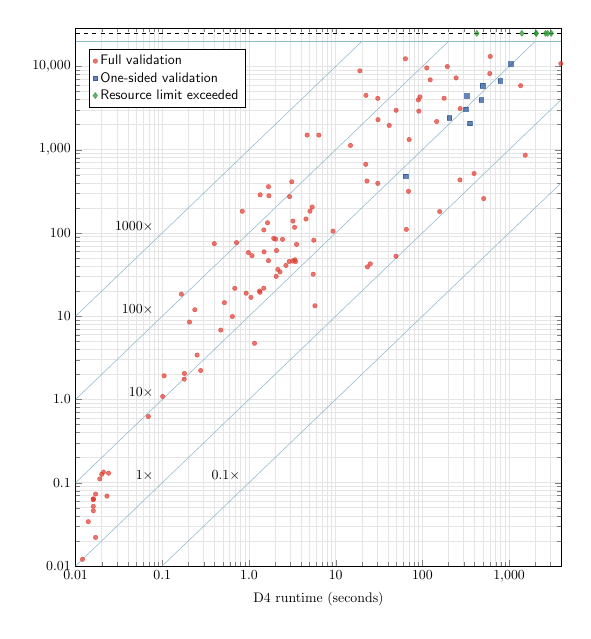
\begin{tikzpicture}[scale = 0.50]
  \begin{axis}[mark options={scale=0.55},grid=both, grid style={black!10}, ymode=log,
      legend style={at={(0.35,0.96)}},
      legend cell align={left},
                              x post scale=1.8, y post scale=2.4,
                              xmode=log,xmin=0.01,xmax=4000,
                              xtick={0.01, 0.1,1.0,10,100,1000,10000}, xticklabels={0.01, 0.1, 1.0, 10, 100, {1,000}, {10,000}},
                              ymin=0.01, ymax=29000,
                              ytick={0.01, 0.1,1.0,10,100,1000,10000,100000}, yticklabels={0.01, 0.1, 1.0, 10, 100, {1,000},{10,000},{100,000}},
                              xlabel={D4 runtime (seconds)},
                              %ylabel={CPOG generation and checking runtime (seconds)},
%                              title={D4 Defining Clause Generation}
            ]
%    \input{data-formatted/time-d4-verify}

\addplot [only marks, color=redorange, mark=*,  mark options={scale=0.8}, opacity=0.7] coordinates { (5.758,13.334) (0.017,0.022) (0.014,0.034) (0.179,1.754) (0.016,0.046) (0.012,0.012) (0.024,0.13) (0.928,18.877) (0.069,0.624) (0.166,18.378) (1.48,21.674999999999997) (3.356,116.882) (3.184,46.001000000000005) (1.676,46.439) (0.016,0.063) (0.019,0.11100000000000002) (0.472,6.808) (0.02,0.126) (5.048,182.556) (0.398,74.411) (0.685,21.603) (0.252,3.414) (30.753,2292.7690000000002) (0.643,9.902) (2.154,36.441) (1.158,4.7219999999999995) (2.436,83.753) (1.636,132.504) (1.491,59.292) (4.683,1499.441) (30.566,4136.219) (145.967,2177.9669999999996) (2.666,40.712) (0.105,1.923) (5.508,31.97) (244.952,7273.887000000001) (0.206,8.503) (606.378,13198.325) (23.234,39.160000000000004) (0.837,182.089) (49.574,52.467) (25.077,42.550000000000004) (63.691,12374.461) (4.544,147.119) (1.679,359.63) (22.322,4493.414000000001) (2.076,61.509) (70.355,1322.4) (90.915,2908.19) (123.037,6910.268) (112.248,9602.115) (178.14,4147.301) (394.71,517.646) (158.115,180.629) (69.122,315.91) (508.972,258.496) (2.033,84.352) (270.954,433.669) (1536.914,859.557) (19.013,8856.852) (2.938,272.899) (598.709,8218.087) (9.311,105.213) (0.277,2.226) (0.101,1.086) (30.577,394.01700000000005) (0.18,2.051) (0.016,0.064) (0.021,0.134) (0.52,14.541) (0.016,0.063) (0.237,11.949000000000002) (0.985,58.088) (2.278,33.982) (1.053,16.815) (1.326,20.087) (2.908,45.419) (3.441,45.275) (2.06,30.061999999999998) (1.483,108.72) (3.377,47.61) (0.017,0.073) (0.016,0.052000000000000005) (3.536,72.871) (1.337,19.372999999999998) (5.587,81.767) (193.799,9953.933) (89.858,3959.588) (0.023,0.06899999999999999) (49.796,2973.447) (0.718,76.449) (5.364,204.765) (3.21,138.828) (41.455,1955.3980000000001) (1.083,53.278999999999996) (1.695,279.8) (1.345,286.818) (3.111,411.545) (6.397,1495.882) (22.214,666.7180000000001) (65.322,110.378) (22.917,420.612) (272.642,3116.728) (1.929,85.946) (1358.165,5872.383) (3951.002,10810.879) (14.808,1124.911) (93.537,4307.451)};

%    \input{data-formatted/time-d4-verify-onesided-only}

\addplot [only marks, color=bluegray, mark=square*,  mark options={scale=0.8}, opacity=0.7] coordinates { (205.743,2420.6859999999997) (326.575,4433.625) (476.021,3973.2659999999996) (494.38,5879.952) (1046.603,10779.982) (351.999,2069.865) (64.21,479.92100000000005) (316.505,3074.084) (788.377,6710.351000000001)};

%    \input{data-formatted/time-d4-failure}

\addplot [only marks, color=darkgreen, mark=diamond*, mark options={scale=1.1}, opacity=0.7] coordinates { (2052.239,25000) (424.73,25000) (2636.562,25000) (1403.431,25000) (3070.214,25000) (2053.446,25000) (2790.169,25000)};


    \legend{
 \textsf{Full validation},
 \textsf{One-sided validation},
 \textsf{Resource limit exceeded},
    }
    \addplot[mark=none, dashed] coordinates{(0.01,25000) (4000, 25000)};
    \addplot[mark=none, color=lightblue] coordinates{(0.01,20000) (4000,20000)};
    \addplot[mark=none, color=lightblue] coordinates{(0.1,0.01) (10000.0,1000.0)};
    \addplot[mark=none, color=lightblue] coordinates{(0.01,0.01) (10000.0,10000.0)};
    \addplot[mark=none, color=lightblue] coordinates{(0.01,0.1) (2000,20000)};
    \addplot[mark=none, color=lightblue] coordinates{(0.01,1.0) (200, 20000)};
    \addplot[mark=none, color=lightblue] coordinates{(0.01,10.0) (20, 20000)};
    \node[left] at (axis cs: 0.9,0.12) {$0{.}1\times$};
    \node[left] at (axis cs: 0.09,0.12) {$1\times$};
    \node[left] at (axis cs: 0.09,1.2) {$10\times$};
    \node[left] at (axis cs: 0.09,12.0) {$100\times$};
    \node[left] at (axis cs: 0.09,120.0) {$1000\times$};

          \end{axis}
\end{tikzpicture}
} % centering
\end{minipage}
\begin{minipage}{0.49\textwidth}
\centering{%
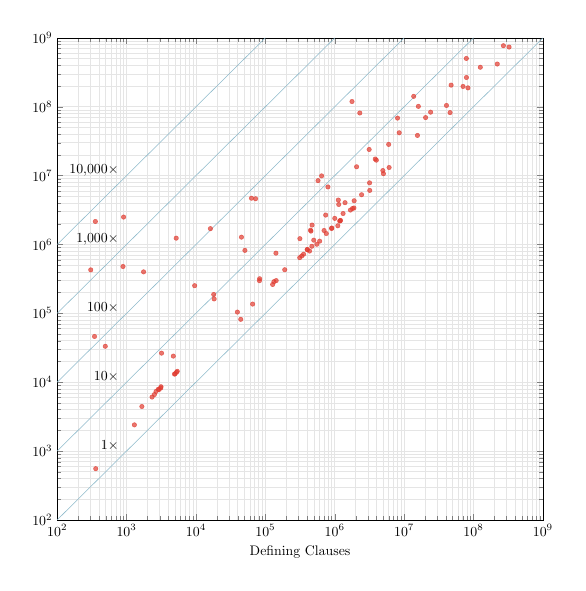
\begin{tikzpicture}[scale = 0.50]
  \begin{axis}[mark options={scale=0.55},grid=both, grid style={black!10},
                              x post scale=1.8, y post scale=2.15,
                              xmode=log,xmin=100,xmax=1000000000, 
                              xtick={100,1000, 10000, 100000, 1000000, 10000000, 100000000, 1000000000}, xticklabels={$10^2$,$10^3$,$10^4$,$10^5$,$10^6$,$10^7$,$10^8$,$10^9$},
                              ymode=log, ymin=100, ymax=1000000000, 
                              ytick={100,1000, 10000, 100000, 1000000, 10000000, 100000000, 1000000000}, yticklabels={$10^2$,$10^3$,$10^4$,$10^5$,$10^6$,$10^7$,$10^8$,$10^9$},
                              xlabel={Defining Clauses},
                              %ylabel={Proof Clauses},
%                              title={D4 Defining Clause Generation}
            ]
    \addplot[mark=none, color=lightblue] coordinates{(100,100) (1e9,1e9)};
    \addplot[mark=none, color=lightblue] coordinates{(100,1000) (1e8,1e9)};
    \addplot[mark=none, color=lightblue] coordinates{(100,10000) (1e7,1e9)};
    \addplot[mark=none, color=lightblue] coordinates{(100,100000) (1e6,1e9)};
    \addplot[mark=none, color=lightblue] coordinates{(100,1000000) (1e5,1e9)};
%%    \input{data-formatted/defining+total}

\addplot [only marks, color=redorange, mark=*,  mark options={scale=0.8}, opacity=0.7] coordinates { (18271,161794) (1295,2397) (1659,4427) (127284,262373) (2325,6077) (359,554) (5373,14373) (314359,1213826) (44178,81780) (493,33207) (605988,1117440) (1141369,3809317) (1197649,2211944) (1001050,2393131) (2947,7851) (4991,13207) (355617,721935) (4897,13101) (2437497,5273728) (345,46079) (701346,1593947) (3191,26378) (5985623,28392373) (467550,940819) (1318024,2813565) (4713,23892) (1682059,3160386) (1406192,4043887) (899701,1704811) (4936014,11840667) (8038928,68469623) (70651620,197339867) (9567,251890) (39501,104182) (18007,187551) (125319627,374762287) (82194,297768) (269645146,770382773) (304,427342) (574062,8448281) (887,478450) (1757,399856) (78873354,503117290) (190248,429409) (2064844,13434107) (13737124,141587875) (50722,820648) (45923418,82243431) (83111464,188103550) (40776253,104351646) (79106742,265990284) (3133905,23973053) (16147,1697847) (45214,1277037) (72258,4612352) (905,2500003) (401032,840020) (355,2155900) (63050,4692737) (3195277,6098685) (1125105,4417869) (325251378,736764776) (6074672,13104909) (132891,287958) (65522,136116) (15561156,38336288) (143191,298755) (2851,7851) (5243,13911) (334862,681444) (2659,7335) (82585,317789) (447979,1612224) (905899,1733678) (433226,802268) (551970,1006319) (1891045,3387533) (1210098,2232426) (755273,1440924) (470934,1914084) (1178453,2188886) (3131,8575) (2515,6607) (1903735,4312279) (1107098,1868005) (1801878,3324418) (47556240,206213289) (24087642,83491057) (3109,8227) (16038150,101261480) (312728,642675) (3175308,7847036) (142059,747752) (20382514,69650789) (453769,1563728) (498246,1154507) (797866,6840229) (3835114,17412807) (5035130,10668725) (647011,9905453) (5189,1234644) (740235,2672407) (219979530,417455256) (402460,844395) (2295530,81147729) (1772352,119113610) (3975194,16763326) (8493275,41873955)};


    \node[left] at (axis cs: 900,1200) {$1\times$};
    \node[left] at (axis cs: 900,12000) {$10\times$};
    \node[left] at (axis cs: 900,120000) {$100\times$};
    \node[left] at (axis cs: 900,1200000) {$1{,}000\times$};
    \node[left] at (axis cs: 900,12000000) {$10{,}000\times$};

          \end{axis}
\end{tikzpicture}
} % centering
\end{minipage}
\caption{Runtime (left) and proof size (right) for CPOG proofs.  The runtime includes proof generation, checking, and model counting relative to the runtime for D4.
  The proof size is measured as total clauses relative to the number of defining clauses.}
\label{fig:dual:total}
\end{figure}


We summarize the results of our experiments here.
The supplement~\cite{bryant:sat:2023:supplement}
provides a more complete description. For our
evaluation, we used the public benchmark problems from the 2022
standard and weighted model competitions.\footnote{Downloaded from \url{https://mccompetition.org/2022/mc\_description.html}}  We found that there were
180 unique CNF files among these, ranging in size from 250 to
2,753,207 clauses.
We ran our programs on a processor with 64~GB of
memory and having an attached high-speed, solid-state
disk.
With a runtime limit of 4000 seconds, \dfour{} completed for 124 of the
benchmark problems.  Our proof generator was able to convert all of
these into POGs, with their declarations ranging from 304 to
2,761,457,765 (median 848,784) defining clauses.
%(The
%maximum count overflowed the overflowed the 32-bit signed integers we
%used to represent clause identifiers in both the proof generator and
%checker.)

We ran our proof generator with a time limit of 10,000 seconds.  The
results are shown in Figure~\ref{fig:dual:total}, The left-hand plot
shows the elapsed time for the combination of proof generation,
checking, and counting versus the time for
\dfour{}.
The proof generator was able to generate full proofs for 108 of the problems and
one-sided proofs for an additional 9 of them, leaving just 7 with no
verification.  The prototype checker successfully verified all of the generated
proofs.  The longest runtime for the combination of proof generation, checking, and counting
for a full proof was 13,145 seconds.
Overall the ratio
between the combined time for generation, checking, and counting versus the time
for \dfour{} had a harmonic mean of 5.5.
The right-hand plot shows the total number of clauses in the CPOG file versus the number of defining clauses for the problems having full proofs.
The ratio between the total number of clauses and the number of defining clauses had a harmonic mean of 3.13.
To date, we have not found
any errors in the dec-DNNF graphs generated by \dfour{}.

We found that the monolithic approach for generating the forward
implication proof works well for smaller POGs (up to one million
defining clauses), but it becomes inefficient for larger ones.  These
experiments suggest a possible hybrid approach, stopping the recursion
of the structural approach and shifting to monolithic mode once the
subgraph size is below some threshold.  By using monolithic mode, we
were also able to perform end-to-end verification of all but one of the
benchmarks that could be verified without preprocessing, with a total
time limit (including preprocessing) of 1,000 seconds.

We also found that our two optimizations: literal grouping and
lemmas can provide substantial improvements in proof size and runtime.
In the extreme cases, a lack
of lemmas caused one proof to grow by a factor of 52.5, while a lack
of literal grouping caused another proof to grow by a factor of 39.6.
Overall, it is clear that these two optimizations are worthwhile, and
sometimes critical, to success for some benchmarks.

Running the verified proof checker in \lean{} required, on average
(harmonic mean), around 5.9 times longer than the prototype checker.
Encouragingly, the scaling trends were identical for the two solvers,
indicating that the two checkers have similar asymptotic performance.
We consider a factor of 5.9 to be acceptable for the assurance
provided by formal verification.

In comparing other proof frameworks, we found that the \cdfour{}
toolchain ran very fast and could handle very large benchmarks.  Even
with a total time limit of 1,000 seconds, including the time for
knowledge compilation, the \cdfour{} toolchain completed 106
benchmarks, while the CPOG toolchain completed just 82.  We found
that the runtimes for the MICE toolchain versus our CPOG toolchain
showed little correlation, reflecting the fact that the two solve
different problems and use different approaches.  In general, our CPOG
toolchain showed better scaling, in part due to its ability to control
the recursion through lemmas.  Neither of these prior
toolchains could perform end-to-end verification when the knowledge
compilation was preceded by preprocessing.

\section{Conclusions}
\label{sect:future}

This paper demonstrates a method for certifying the equivalence of two
different representations of a Boolean formula: an input formula
represented in conjunctive normal form, and a compiled representation
that can then be used to extract useful information about the formula,
including its weighted and unweighted model counts.  It builds on the
extensive techniques that have been developed for clausal
proof systems, including extended resolution and reverse unit propagation, as well as established tools, such as
proof-generating SAT solvers and \dtrim{}.


We are hopeful that having checkable proofs for knowledge compilers
will allow them to be used in applications where high levels of trust
are required, and that it will provide a useful tool for developers of
knowledge compilers.
%%Although our current implementation only handles
%%the outputs of one particular program, it could be adapted
Our experiments demonstrate that our toolchain can already handle
problems nearly at the limits of current knowledge compilers.  Further
engineering and optimization of our proof generator and checker could
improve their performance and capacity substantially.  We are hopeful
that our tool can be adapted to handle other knowledge compiler
representations, such as sentential decision diagrams (SDDs)~\cite{darwiche:ijcai:2011}.


%% Each node $\nodeu$ in an $SDD$ has children $p_1, p_2, \ldots, p_k$ and
%% $s_1, s_2, \ldots p_k$, where the Boolean formula $\phi(\nodeu)$ associated
%% with the node is defined recursively as $\phi(\nodeu) = \bigwedge_{1 \leq i \leq k}
%% [\phi(p_i) \land \phi(s_i)]$.  Moreover, each children $p_i$ and $p_j$
%% such that $1 \leq i < j \leq k$ must satisfy $\modelset(\phi(p_i))
%% \cap \modelset(\phi(p_j)) = \emptyset$, and for every $p_i$ and $s_j$
%% such that $1 \leq i,j \leq k$, we must have $\dependencyset(\phi(p_i))
%% \cap \dependencyset(\phi(s_j)) = \emptyset$.  The POG representation
%% of such a node could have $k$ product nodes: $t_i = p_i \pand s_i$
%% for $1 \leq i \leq k$, and then $k-1$ binary sum nodes to form
%% the sum of $t_1, \ldots, t_k$.

%%\newpage


\bibliography{references}
\bibliographystyle{theapa}

\end{document}
